\documentclass[11pt,a4paper,]{article}
\usepackage{lmodern}

\usepackage{amssymb,amsmath}
\usepackage{ifxetex,ifluatex}
\usepackage{fixltx2e} % provides \textsubscript
\ifnum 0\ifxetex 1\fi\ifluatex 1\fi=0 % if pdftex
  \usepackage[T1]{fontenc}
  \usepackage[utf8]{inputenc}
\else % if luatex or xelatex
  \usepackage{unicode-math}
  \defaultfontfeatures{Ligatures=TeX,Scale=MatchLowercase}
\fi
% use upquote if available, for straight quotes in verbatim environments
\IfFileExists{upquote.sty}{\usepackage{upquote}}{}
% use microtype if available
\IfFileExists{microtype.sty}{%
\usepackage[]{microtype}
\UseMicrotypeSet[protrusion]{basicmath} % disable protrusion for tt fonts
}{}
\PassOptionsToPackage{hyphens}{url} % url is loaded by hyperref
\usepackage[unicode=true]{hyperref}
\hypersetup{
            pdftitle={A fast and elegant method for forecast reconciliation using linear forecasting models},
            pdfkeywords={hierarchical forecasting, grouped forecasting, reconciling forecast, linear regression},
            pdfborder={0 0 0},
            breaklinks=true}
\urlstyle{same}  % don't use monospace font for urls
\usepackage{geometry}
\geometry{left=2.5cm,right=2.5cm,top=2.5cm,bottom=2.5cm}
\usepackage[style=authoryear-comp,]{biblatex}
\addbibresource{references.bib}
\usepackage{longtable,booktabs}
% Fix footnotes in tables (requires footnote package)
\IfFileExists{footnote.sty}{\usepackage{footnote}\makesavenoteenv{long table}}{}
\IfFileExists{parskip.sty}{%
\usepackage{parskip}
}{% else
\setlength{\parindent}{0pt}
\setlength{\parskip}{6pt plus 2pt minus 1pt}
}
\setlength{\emergencystretch}{3em}  % prevent overfull lines
\providecommand{\tightlist}{%
  \setlength{\itemsep}{0pt}\setlength{\parskip}{0pt}}
\setcounter{secnumdepth}{5}

% set default figure placement to htbp
\makeatletter
\def\fps@figure{htbp}
\makeatother


\title{A fast and elegant method for forecast reconciliation using linear forecasting models}

%% MONASH STUFF

%% CAPTIONS
\RequirePackage{caption}
\DeclareCaptionStyle{italic}[justification=centering]
 {labelfont={bf},textfont={it},labelsep=colon}
\captionsetup[figure]{style=italic,format=hang,singlelinecheck=true}
\captionsetup[table]{style=italic,format=hang,singlelinecheck=true}

%% FONT
\RequirePackage{bera}
\RequirePackage{mathpazo}

%% HEADERS AND FOOTERS
\RequirePackage{fancyhdr}
\pagestyle{fancy}
\rfoot{\Large\sffamily\raisebox{-0.1cm}{\textbf{\thepage}}}
\makeatletter
\lhead{\textsf{\expandafter{\@title}}}
\makeatother
\rhead{}
\cfoot{}
\setlength{\headheight}{15pt}
\renewcommand{\headrulewidth}{0.4pt}
\renewcommand{\footrulewidth}{0.4pt}
\fancypagestyle{plain}{%
\fancyhf{} % clear all header and footer fields
\fancyfoot[C]{\sffamily\thepage} % except the center
\renewcommand{\headrulewidth}{0pt}
\renewcommand{\footrulewidth}{0pt}}

%% MATHS
\RequirePackage{bm,amsmath}
\allowdisplaybreaks

%% GRAPHICS
\RequirePackage{graphicx}
\setcounter{topnumber}{2}
\setcounter{bottomnumber}{2}
\setcounter{totalnumber}{4}
\renewcommand{\topfraction}{0.85}
\renewcommand{\bottomfraction}{0.85}
\renewcommand{\textfraction}{0.15}
\renewcommand{\floatpagefraction}{0.8}

%\RequirePackage[section]{placeins}

%% SECTION TITLES
\RequirePackage[compact,sf,bf]{titlesec}
\titleformat{\section}[block]
  {\fontsize{15}{17}\bfseries\sffamily}
  {\thesection}
  {0.4em}{}
\titleformat{\subsection}[block]
  {\fontsize{12}{14}\bfseries\sffamily}
  {\thesubsection}
  {0.4em}{}
\titlespacing{\section}{0pt}{*5}{*1}
\titlespacing{\section}{0pt}{*2}{*0.2}


%% TITLE PAGE
\def\Date{\number\day}
\def\Month{\ifcase\month\or
 January\or February\or March\or April\or May\or June\or
 July\or August\or September\or October\or November\or December\fi}
\def\Year{\number\year}

\makeatletter
\def\wp#1{\gdef\@wp{#1}}\def\@wp{??/??}
\def\jel#1{\gdef\@jel{#1}}\def\@jel{??}
\def\showjel{{\large\textsf{\textbf{JEL classification:}}~\@jel}}
\def\nojel{\def\showjel{}}
\def\addresses#1{\gdef\@addresses{#1}}\def\@addresses{??}
\def\cover{{\sffamily\setcounter{page}{0}
        \thispagestyle{empty}%
        \vspace*{-2cm}
        \centerline{\raisebox{-1.8cm}{
\includegraphics[width=5cm]{MBSportrait}}\hspace*{9cm} ISSN 1440-771X}\vspace{0.99cm}
        \begin{center}\Large
        Department of Econometrics and Business Statistics\\[.5cm]
        \scriptsize http://business.monash.edu/econometrics-and-business-statistics/research/publications
        \end{center}\vspace{2cm}
        \begin{center}
        \fbox{\parbox{14cm}{\begin{onehalfspace}\centering\Huge\vspace*{0.3cm}
                \textsf{\textbf{\expandafter{\@title}}}\vspace{1cm}\par
                \LARGE\@author\end{onehalfspace}
        }}
        \end{center}
        \vfill
                \begin{center}\Large
                \Month~\Year\\[1cm]
                Working Paper \@wp
        \end{center}}}
\def\pageone{{\sffamily\setstretch{1}%
        \thispagestyle{empty}%
        \vbox to \textheight{%
        \raggedright\baselineskip=1.2cm
     {\fontsize{24.88}{30}\sffamily\textbf{\expandafter{\@title}}}
        \vspace{2cm}\par
        \hspace{1cm}\parbox{14cm}{\sffamily\large\@addresses}\vspace{1cm}\vfill
        \hspace{1cm}{\large\Date~\Month~\Year}\\[1cm]
        \hspace{1cm}\showjel\vss}}}
\def\blindtitle{{\sffamily
     \thispagestyle{plain}\raggedright\baselineskip=1.2cm
     {\fontsize{24.88}{30}\sffamily\textbf{\expandafter{\@title}}}\vspace{1cm}\par
        }}
\def\titlepage{{\cover\newpage\pageone\newpage\blindtitle}}

\def\blind{\def\titlepage{{\blindtitle}}\let\maketitle\blindtitle}
\def\titlepageonly{\def\titlepage{{\pageone\end{document}}}}
\def\nocover{\def\titlepage{{\pageone\newpage\blindtitle}}\let\maketitle\titlepage}
\let\maketitle\titlepage
\makeatother

%% SPACING
\RequirePackage{setspace}
\spacing{1.5}

%% LINE AND PAGE BREAKING
\sloppy
\clubpenalty = 10000
\widowpenalty = 10000
\brokenpenalty = 10000
\RequirePackage{microtype}

%% PARAGRAPH BREAKS
\setlength{\parskip}{1.4ex}
\setlength{\parindent}{0em}

%% HYPERLINKS
\RequirePackage{xcolor} % Needed for links
\definecolor{darkblue}{rgb}{0,0,.6}
\RequirePackage{url}

\makeatletter
\@ifpackageloaded{hyperref}{}{\RequirePackage{hyperref}}
\makeatother
\hypersetup{
     citecolor=0 0 0,
     breaklinks=true,
     bookmarksopen=true,
     bookmarksnumbered=true,
     linkcolor=darkblue,
     urlcolor=blue,
     citecolor=darkblue,
     colorlinks=true}

%% KEYWORDS
\newenvironment{keywords}{\par\vspace{0.5cm}\noindent{\sffamily\textbf{Keywords:}}}{\vspace{0.25cm}\par\hrule\vspace{0.5cm}\par}

%% ABSTRACT
\renewenvironment{abstract}{\begin{minipage}{\textwidth}\parskip=1.4ex\noindent
\hrule\vspace{0.1cm}\par{\sffamily\textbf{\abstractname}}\newline}
  {\end{minipage}}


\usepackage[T1]{fontenc}
\usepackage[utf8]{inputenc}

\usepackage[showonlyrefs]{mathtools}
\usepackage[no-weekday]{eukdate}

%% BIBLIOGRAPHY

\makeatletter
\@ifpackageloaded{biblatex}{}{\usepackage[style=authoryear-comp, backend=biber, natbib=true]{biblatex}}
\makeatother
\ExecuteBibliographyOptions{bibencoding=utf8,minnames=1,maxnames=3, maxbibnames=99,dashed=false,terseinits=true,giveninits=true,uniquename=false,uniquelist=false,doi=false, isbn=false,url=true,sortcites=false}

\DeclareFieldFormat{url}{\texttt{\url{#1}}}
\DeclareFieldFormat[article]{pages}{#1}
\DeclareFieldFormat[inproceedings]{pages}{\lowercase{pp.}#1}
\DeclareFieldFormat[incollection]{pages}{\lowercase{pp.}#1}
\DeclareFieldFormat[article]{volume}{\mkbibbold{#1}}
\DeclareFieldFormat[article]{number}{\mkbibparens{#1}}
\DeclareFieldFormat[article]{title}{\MakeCapital{#1}}
\DeclareFieldFormat[article]{url}{}
%\DeclareFieldFormat[book]{url}{}
%\DeclareFieldFormat[inbook]{url}{}
%\DeclareFieldFormat[incollection]{url}{}
%\DeclareFieldFormat[inproceedings]{url}{}
\DeclareFieldFormat[inproceedings]{title}{#1}
\DeclareFieldFormat{shorthandwidth}{#1}
%\DeclareFieldFormat{extrayear}{}
% No dot before number of articles
\usepackage{xpatch}
\xpatchbibmacro{volume+number+eid}{\setunit*{\adddot}}{}{}{}
% Remove In: for an article.
\renewbibmacro{in:}{%
  \ifentrytype{article}{}{%
  \printtext{\bibstring{in}\intitlepunct}}}

\AtEveryBibitem{\clearfield{month}}
\AtEveryCitekey{\clearfield{month}}

\makeatletter
\DeclareDelimFormat[cbx@textcite]{nameyeardelim}{\addspace}
\makeatother
\renewcommand*{\finalnamedelim}{%
  %\ifnumgreater{\value{liststop}}{2}{\finalandcomma}{}% there really should be no funny Oxford comma business here
  \addspace\&\space}


\wp{no/yr}
\jel{C10,C14,C22}

\nocover

\author{Mahsa~Ashouri, Rob J~Hyndman, Galit~Shmueli}
\addresses{\textbf{Mahsa Ashouri}\newline
Institute of Service Science, National Tsing Hua University, Taiwan
\newline{Email: \href{mailto:mahsa.ashouri@iss.nthu.edu.tw}{\nolinkurl{mahsa.ashouri@iss.nthu.edu.tw}}}\newline Corresponding author\\[1cm]
\textbf{Rob J Hyndman}\newline
Monash University, Clayton VIC 3800, Australia
\newline{Email: \href{mailto:rob.hyndman@monash.edu}{\nolinkurl{rob.hyndman@monash.edu}}}\\[1cm]
\textbf{Galit Shmueli}\newline
Institute of Service Science, National Tsing Hua University, Taiwan
\newline{Email: \href{mailto:galit.shmueli@iss.nthu.edu.tw}{\nolinkurl{galit.shmueli@iss.nthu.edu.tw}}}\\[1cm]
}

\date{\sf\Date~\Month~\Year}
\makeatletter
 \lfoot{\sf Ashouri, Hyndman, Shmueli: \@date}
\makeatother

%% Any special functions or other packages can be loaded here.

\usepackage{booktabs}
\usepackage{float}
\usepackage{longtable}
\usepackage{cases}
\usepackage{array}
\usepackage{todonotes}
%\usepackage[backend=biber]{biblatex}
%\usepackage[backend=biber, bibencoding=utf8, style=authoryear, citestyle=authoryear]{biblatex}


\begin{document}
\maketitle
\begin{abstract}
Forecasting hierarchical or grouped time series involves two steps: computing base forecasts and reconciling the forecasts. Base forecasts can be computed by popular time series forecasting methods such as Exponential Smoothing (ETS) and Autoregressive Integrated Moving Average (ARIMA) models. The reconciliation step is a linear process that adjusts the base forecasts to ensure they are coherent. However using ETS or ARIMA for base forecasts can be computationally challenging when there are a large number of series to forecast, as each model must be numerically optimized for each series. We propose a linear model that avoids this computational problem, and uses a single-step approach to obtain the forecasts, rather than the usual two-step approach. The proposed method is very flexible in incorporating external data and handling missing values. We illustrate our approach using two datasets: monthly Australian domestic tourism and daily Wikipedia pageviews. We compare our approach to reconciliation using ETS and ARIMA, and show that our approach is much faster while providing similar levels of forecast accuracy.
\end{abstract}
\begin{keywords}
hierarchical forecasting, grouped forecasting, reconciling forecast, linear regression
\end{keywords}

\hypertarget{introduction}{%
\section{Introduction}\label{introduction}}

Modern data collection tools have dramatically increased the amount of available time series data. For example, the Internet of Things (IoT) and point-of-sale scanning produce huge volumes of time series in a short period of time. Naturally, there is an interest in forecasting these time series, yet forecasting large collections of time series is computationally challenging.

\hypertarget{hierarchical-and-grouped-time-series}{%
\subsection{Hierarchical and grouped time series}\label{hierarchical-and-grouped-time-series}}

In many cases, these time series can be structured and disaggregated based on hierarchies or groups such as geographic location, product type, gender, etc. An example of hierarchical time series is sales in restaurant chains, which can be disaggregated into different stores and then different types of food or drinks. Figure \ref{fig:hierarchicalexample} shows a schematic of such a hierarchical time series structure with three levels. The top level (level 0) is the total series, formed by aggregating all the bottom level series. In the middle level (level 1), series are aggregations of their own child series; for instance, series A is the aggregation of AA and AB. Finally, the bottom level series (level 2), includes the most disaggregated series.

\begin{figure}

{\centering 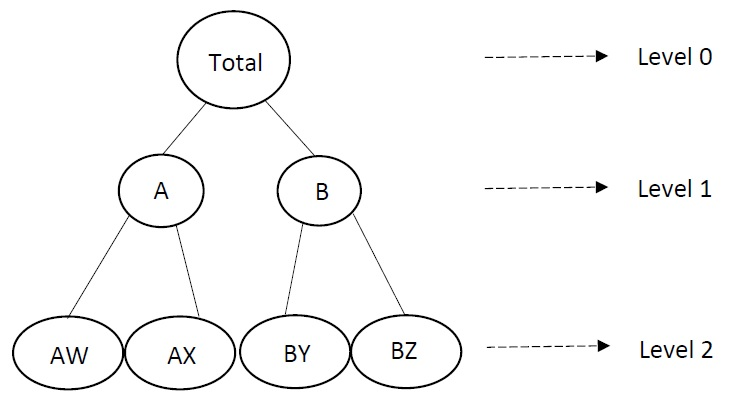
\includegraphics[width=280px,height=180px]{Paper-Figures/hierarchical_example} 

}

\caption{An example of a two level hierarchy structure}\label{fig:hierarchicalexample}
\end{figure}

\begin{figure}

{\centering 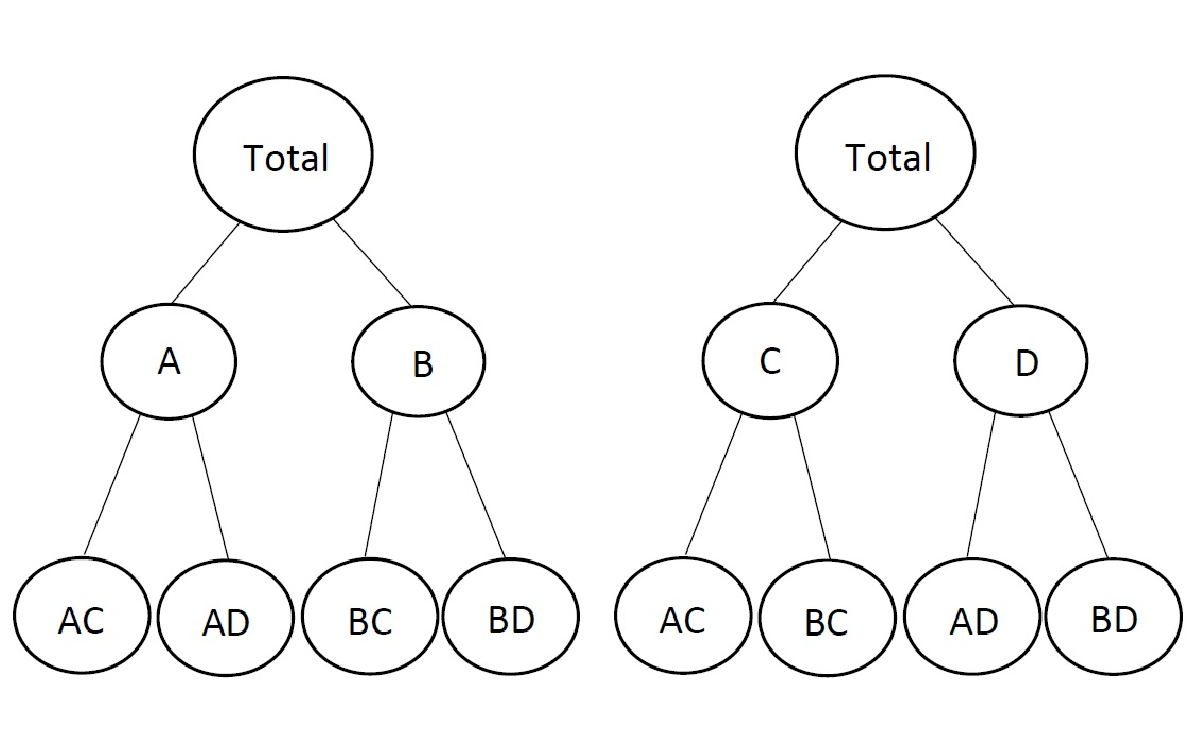
\includegraphics[width=280px,height=180px]{hcf_files/figure-latex/groupexample-1} 

}

\caption{An example of two level grouped structure}\label{fig:groupexample}
\end{figure}

Grouped time series involve more complicated aggregation structures compared to strictly hierarchical time series. To take the simplest example, suppose we have two grouping factors which are not nested; for example, sex (Male/Female) and city (New York/San Francisco). The disaggregated series for each combination of sex and city can be combined to form city sub-totals, or sex sub-totals. These sub-totals can be combined to give the overall total. Both sub-totals are of interest.

We can think of such structures as hierarchical time series without a unique hierarchy. A schematic of this grouped time series structure is shown in Figure \ref{fig:groupexample} with two grouping factors, each of two levels (A/B and C/D). The series in this structure can be split first into groups A and B and then subdivided further into C and D (left side), or split first into C and D and then subdivided into A and B (right side). The final disaggregation is identical in both cases, but the middle level aggregates are different.

We use the same notation \autocite[following][]{fpp2} for both hierarchical and grouped time series. We denote the total series at time \(t\) by \(y_t\), and the series at node \(Z\) and time \(t\) by \(y_{Z,t}\). For describing the relationships between series, we use an \(n\times m\) matrix, called the `summing matrix', denoted by \(\bm{S}\), in which \(n\) is the overall number of nodes and \(m\) is the number of bottom level nodes. For example in Figure \ref{fig:hierarchicalexample}, \(n = 7\) and \(m = 4\), while in Figure \ref{fig:groupexample}, \(n=9\) and \(m=4\). Then we can write \(\bm{y}_t=\bm{S}\bm{b}_t\), where \(\bm{y}_t\) is a vector of all the level nodes at time \(t\) and \(\bm{b}_t\) is the vector of all the bottom level nodes at time \(t\). For the example shown in Figure \ref{fig:groupexample}, the equation can be written as follows:
\begin{equation}\label{eq:Smatrixexample}
\begin{pmatrix}
  y_{t}\\y_{A,t}\\y_{B,t}\\y_{C,t}\\y_{D,t}\\y_{AC,t}\\y_{AD,t}\\y_{BC,t}\\y_{BD,t}
\end{pmatrix} =
\begin{pmatrix}
  1&1&1&1\\1&1&0&0\\0&0&1&1\\1&0&1&0\\0&1&0&1\\1&0&0&0\\0&1&0&0\\0&0&1&0\\0&0&0&1\\
\end{pmatrix}
\begin{pmatrix}
  y_{AC,t}\\y_{AD,t}\\y_{BC,t}\\y_{BD,t}\\
\end{pmatrix}
\end{equation}

\hypertarget{forecasting-hierarchical-time-series}{%
\subsection{Forecasting hierarchical time series}\label{forecasting-hierarchical-time-series}}

If we just forecast each series individually, we are ignoring the hierarchical or grouping structure, and the forecasts will not be ``coherent'' (they will not add up appropriately).

There are several available methods that consider the hierarchical structure information when forecasting time series. These include the top-down \autocites{gross1990disaggregation}{fliedner2001hierarchical}, bottom-up \autocite{kahn1998revisiting}, middle-out and optimal combination \autocite{hyndman2011optimal} approaches. In the top-down approach, we first forecast the total series and then disaggregate the forecast to form lower level series forecasts based on a set of historical and forecasted proportions \autocite[for details see][]{athanasopoulos2009hierarchical}. In the bottom-up approach, the forecasts in each level of the hierarchy can be computed by aggregating the bottom level series forecasts. However, we may not get good upper-level forecasts because the most disaggregated series are highly noisy and so their forecasts are usually inaccurate. In the middle-out approach, the process can be started from one of the middle levels and other forecasts can be computed using aggregation for upper levels and disaggregation for lower levels. Finally, optimal combination uses all the \(n\) forecasts for all of the series in the entire structure, and then uses an optimization process to reconcile the resulting forecasts. The advantage of the optimal combination method, compared with the other methods, is that it considers all information in the hierarchy, including any correlations among the series.

In the optimal combination method, reconciled forecasts can be computed using \autocite{mint2018}
\begin{equation}\label{mint}
  \tilde{\bm{y}}_{h}=\bm{S}(\bm{S}'\bm{W}_h^{-1}\bm{S})^{-1}\bm{S}'\bm{W}^{-1}\hat{\bm{y}}_h
\end{equation}
where \(\hat{\bm{y}}_h\) represents a vector of \(h\)-step-ahead base forecasts for all levels of the hierarchy, and \(\bm{W}_h\) is the variance matrix of forecast errors for the \(h\)-step-ahead base forecasts.

The most difficult task is to compute \(\bm{W}_h\), but \textcite{mint2018} and \textcite{hyndman2016fast} argue that replacing it by the diagonal of \(\bm{W}_1\) gives good results in practice. This is easy to obtain because it is simply the diagonal matrix comprising the residual variances from each of the base forecasts.

The most computationally challenging part of the optimal combination method is to produce all the base forecasts that make up \(\hat{\bm{y}}_h\). In many applications, there may be thousands or even millions of individual series, and each of them must be forecast independently. The most popular time series forecasting methods such as ETS and ARIMA models \autocite{fpp2} involve non-linear optimization routines to estimate the parameters via Maximum Likelihood Estimation. Usually, multiple models are fitted for each series, and the best is select by minimizing Akaike's Information Citerion \autocite{akaike1998information}. This computational challenges increases with the number of lower level series as well as in the number of aggregations of interest.

We therefore propose a new approach to compute the base forecasts that is both computationally fast while maintaining an acceptable forecasting accuracy level.

\hypertarget{proposed-approach}{%
\section{Proposed approach}\label{proposed-approach}}

Our proposed approach is based on using linear regression models for computing base forecasts. We use \(\bm{X}_{Z}\) to denote the matrix of \(k\) predictors corresponding to the series at node \(Z\). Then we can write
\begin{equation}\label{eq:linearmodel}
  \bm{y}_Z = \bm{X}_Z \bm{\beta}_Z+\bm{\varepsilon}_Z
\end{equation}
where \(\bm{y}_Z = \{y_{Z,1},\dots,y_{Z,T}\}, \bm{\beta}_Z\) is a vector of coefficients and \(\bm{\varepsilon}_Z\) is an error term with mean zero and variance matrix \(\sigma^2_Z\bm{I}\). Then using standard regression results \autocite{SeberLee}, the OLS estimate of \(\bm{\beta}_Z\) is given by
\begin{equation}\label{eq:linearcoefficientstwosteps}
  \hat{\bm{\beta}}_Z = (\bm{X}_{Z}'\bm{X}_Z)^{-1}\bm{X}_Z'\bm{y}_Z,
\end{equation}
and the base forecasts at horizon \(h\) can be written as
\begin{equation}
  \hat{y}_{Z,T+h} = \bm{x}_{Z,T+h}'(\bm{X}_{Z}'\bm{X}_Z)^{-1}\bm{X}_Z'\bm{y}_Z,
\end{equation}
with corresponding variance
\[
\hat\sigma^2\left[1 + \bm{x}_{Z,T+h}'(\bm{X}_{Z}'\bm{X}_Z)^{-1}\bm{x}_{Z,T+h}\right],
\]
where \(\bm{x}_{Z,T+h}\) denotes the \(k\)-vector of predictors for time period \(T+h\) and
\[
\hat\sigma^2 = \frac{1}{T-k-1}(\bm{y}_Z - \bm{X}_Z\hat{\bm{\beta}}_Z)'(\bm{y}_Z - \bm{X}_Z\hat{\bm{\beta}}_Z).
\]

\todo[inline]{Now we need to write this for all $\hat{y}_Z$, perhaps using multivariate linear regression.}

\hypertarget{previous-proposed-approach}{%
\section{Previous proposed approach}\label{previous-proposed-approach}}

Our proposed approach is based on using linear regression models for computing base forecasts. We begin with partitioning the dataset into training and test sets. We denote by \(\bm{y}_t=\{y_1,y_2,\dots,y_t\}\) and \(\bm{y}_h=\{y_{t+1},y_{t+2},\dots,y_h\}\) the vector of time series in the training and test set for \(h\)-step-ahead forecasts in all the levels of hierarchy. The \(h\)-step-ahead base forecasts and reconciled vectors are denoted by \(\hat{\bm{y}}_{h}\) and \(\tilde{\bm{y}}_{h}\), respectively. We also use \(\bm{X}_t\) and \(\bm{X}_h\) to denote the matrices of predictors in the training and test set, respectively.

The linear forecasting Ordinary Least Square (OLS) model is given by:
\begin{equation}\label{eq:linearmodel}
  \bm{y}_t = \bm{X}_t \bm{\alpha}_h+\delta_h,
\end{equation}
where \(\bm{\alpha}_h\) is the vector of coefficients and \(\delta_h\) is the error term with mean zero and constant variance. We can estimate the reconciled coefficients in two ways: in two steps, \textbf{two-step}, or in single step, \textbf{single-step}. The two-step approach we should first estimate \(\bm{\alpha}_h\) using OLS estimation :
\begin{equation}\label{eq:linearcoefficientstwosteps}
  \hat{\bm{\alpha}}_h = (\bm{X}_t'\bm{X}_t)^{-1}\bm{X}_t'\bm{y}_t,
\end{equation}
and then using Equations \eqref{eq:linearcoefficientstwosteps} and \eqref{eq:reconciledforecasts}, we can find the reconciled forecasts:
\begin{equation}\label{eq:reconciledforecaststwosteps}
  \tilde{\bm{y}}_h = \bm{S}(\bm{S}'\bm{S})^{-1}\bm{S}'\bm{X}_h\hat{\bm{\alpha}}_h.
\end{equation}

We can use Equations \eqref{eq:linearcoefficientstwosteps} and \eqref{eq:reconciledforecaststwosteps} to compute the base forecasts using an OLS forecasting model and then to apply the reconciled forecasts. However because both OLS and reconciliation steps are linear, we can combine these two steps and compute the reconciled forecasts in one step:
\begin{equation}\label{eq:reconciledforecastsonestep}
  \tilde{\bm{y}}_h = \bm{S}(\bm{S}'\bm{S})^{-1}\bm{S}'\bm{X}_h(\bm{X}_t'\bm{X}_t)^{-1}\bm{X}_t'\bm{y}_t
\end{equation}
This single-step reconciliation approach is more parsimonious and elegant.

\hypertarget{ols-predictors}{%
\subsection{OLS predictors}\label{ols-predictors}}

As an example of the \(\bm{X}_t\) matrix in Equation \eqref{eq:linearmodel}, we can refer to the set of predictors proposed in \textcite{ashouri2018} for modeling trend, seasonality and autocorrelation by using lagged values (\(y_{t-1}\), \(y_{t-2}\), \dots), trend variables and seasonal dummy variables as a set of predictors in the linear model. Equation \eqref{eq:linearmodelexample} shows a linear equation of this type which models linear trend, additive seasonality with \(m\) seasons, autocorrelation and external data. Here, \(t\) is the running index (\(t=1,2,\dots\)), and \(s_{jt}\) is a dummy variable taking value 1 if time \(t\) (\(j=1, 2, \dots, m\)) is in season \(j\), \(y_{t-k}\) is the \(k\)th lagged value for \(y_t\) and \(z_t\) is the external data. For instance, if we have daily data with day of week seasonality, \(m\) would be 7 (6 seasonal dummies and 7 the violation of lags).
\todo[inline]{This could cause problems with seasonality modelled with both dummies and an AR process. Perhaps use fewer lags than $m$?}
\begin{equation}\label{eq:linearmodelexample}
    y_t = \alpha_0 + \alpha_1 t + \beta_1 s_{1,t} + \beta_2 s_{2,t} + \cdots + \beta_{m-1} s_{m-1,t} + \gamma_1 y_{t-1} + \gamma_2 y_{t-2} + \dots + \gamma_m y_{t-m} + \delta z_t + \varepsilon_t.
\end{equation}

While OLS is popular in practice for forecasting time series, it is often frown upon due to its independence assumption. This can cause issue for parametric inference but is less of a problem for forecasting, in fact it often performs sufficiently well for forecasting as can be seen by its popular use in practice.

\hypertarget{applications}{%
\section{Applications}\label{applications}}

In this section we illustrate our approach two examples, forecasting monthly Australian domestic tourism and forecasting daily Wikipedia pageviews. We compare the forecasting accuracy levels of ETS, ARIMA and the proposed linear OLS forecasting model, with and without the reconciliation step. For comparing these methods we use the average of Root Mean Square Error (RMSE) across all series and also display box and density plots for forecast errors along with the raw forecast errors.

Since we are using time series lags (\(1, \dots, m\)) in the linear forecasting model, we cant forecast multiple steps ahead. We therefore apply two methods for generating \(h\)-step-ahead forecast: In the first model we use 1-step-ahead forecasts and for forecasting the following periods (\(t+2,t+3,\dots\)) we replace the previous periods with the actual values. This value is known to us because it is in the test set. In our applications, we call this approach `1-step-ahead'. In the second method, we again use 1-step-ahead forecasts but for forecasting the following periods we use the earlier forecasted values. In our applications, we call this approach `\(h\)-step-ahead forecast'. We also show the computation challenges in all the methods.

\hypertarget{australian-domestic-tourism}{%
\subsection{Australian domestic tourism}\label{australian-domestic-tourism}}

This dataset has 19 years of monthly visitor nights in Australia by Australian tourists. This measure is used as an indicator of tourism activity \autocite{mint2018}. This data were collected by computer-assisted telephone interviews with 120000, Australians aged 15 and up \autocite[Research tourism][]{researchAustralia2005}. In total this dataset includes 304 time series with length 228 each. The hierarchy and grouping structure for this dataset is made using geographic and purpose of travel information.

In this dataset we have three levels of geographic divisions in Australia. In the first level, Australia was divided into seven `States' including New South Wales (NSW), Victoria (VIC), Queensland (QLD), South Australia (SA), Western Australia (WA), Tasmania (TAS) and Northern Territory (NT). In the second and third levels it is divided into 27 `Zones' and 76 `Regions' (for details about Australia geographic divisions see Figure \ref{fig:Australiahierarchystructure} and Table \ref{tab:Australiageographicaldivision}). For `Purpose' we have four groups: Holiday (Hol), Visiting (Vis), Business (Bis) and Others (Oth). Based on geographic hierarchy and purpose grouping, we end up with 8 levels of hierarchy with 555 series in total. The hierarchy structure which is used in this example includes the following levels:

\begin{itemize}
\tightlist
\item
  Level 0 = Total series
\item
  Level 1 = State
\item
  Level 2 = Zone
\item
  Level 3 = Region
\item
  Level 4 = Purpose
\item
  Level 5 = State \(\times\) Purpose
\item
  Level 6 = Zone \(\times\) Purpose
\item
  Level 7 = bottom level series
\end{itemize}

We report the forecast results for all these hierarchy levels, as well as the average RMSE across all the levels of hierarchy.

In the predictor matrix, for the OLS forecasting model we apply linear trend, 11 dummy variables, and 12 time series lags\footnote{Since the forecasting results are better without the lags, we just use a linear trend and dummy seasonality variables in our linear model for 24-step-ahead model.}. This is intended to capture the monthly seasonality. In addition, before running the model, we partition the data into two parts, training and test sets. We keep the last 24 months periods (2 years) as our test set to forecast and we use the rest as our training set.

\begin{figure}

{\centering 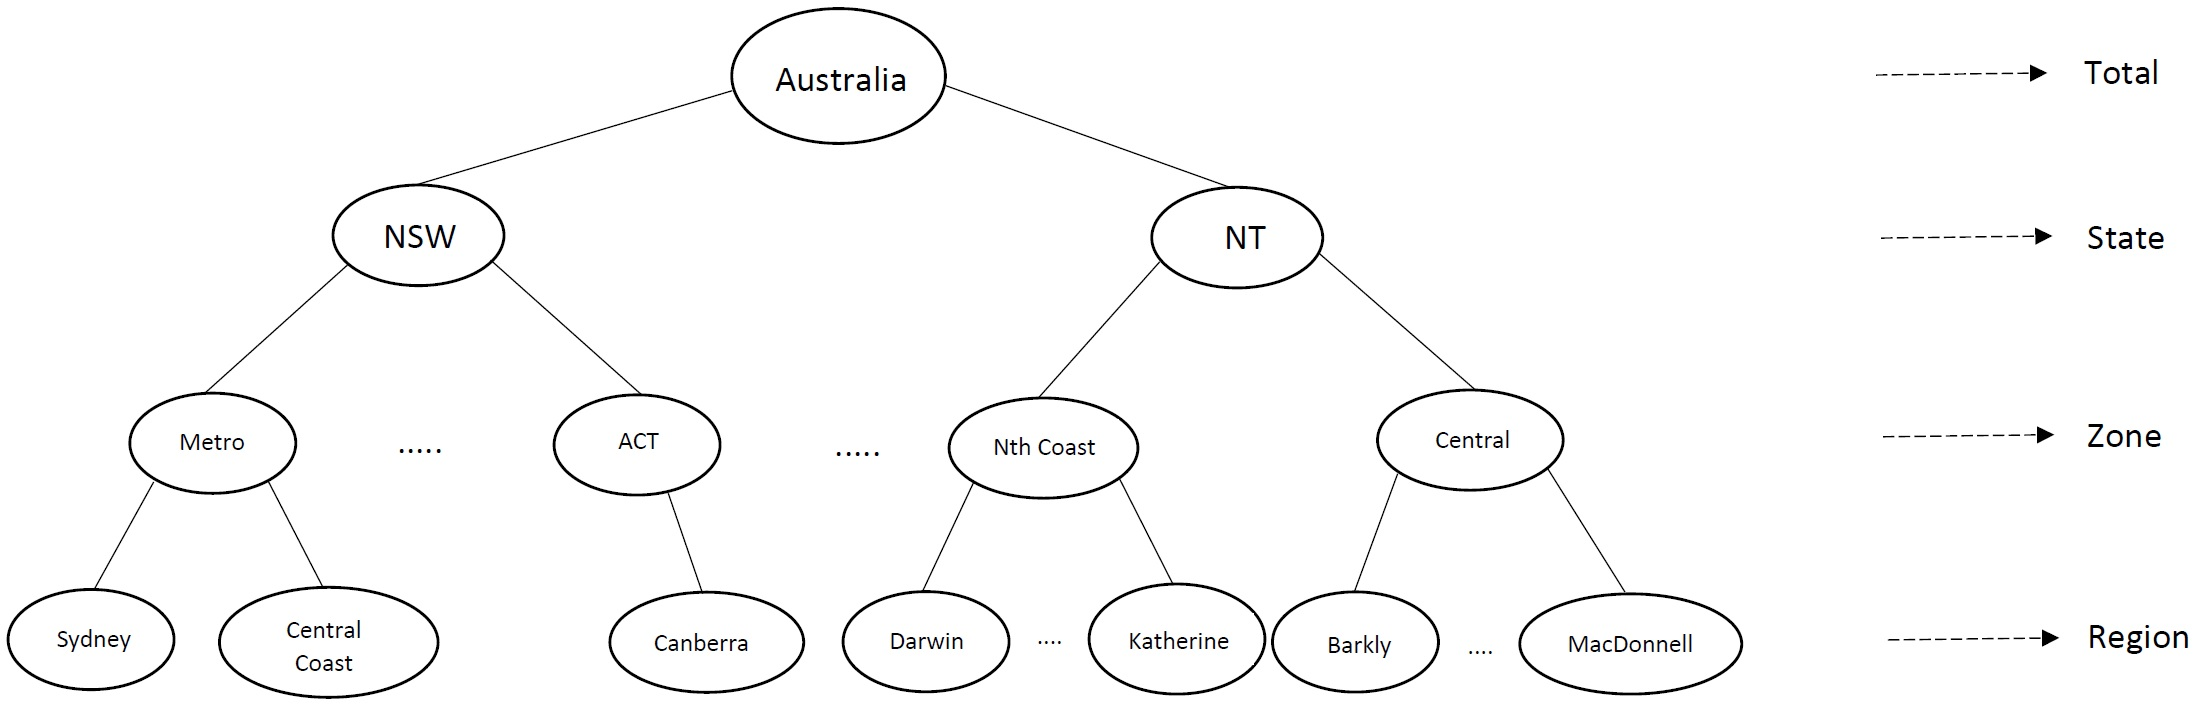
\includegraphics[width=450px,height=180px]{Paper-Figures/Australian_hierarchy_structure} 

}

\caption{Australia geographic hierarchy structure}\label{fig:Australiahierarchystructure}
\end{figure}

\begin{table}[t]

\caption{\label{tab:Australiageographicaldivision}Australia geographic hierarchy structure}
\centering
\fontsize{9}{11}\selectfont
\begin{tabular}{crccrc}
\toprule
Series & Name & Label & Series & Name & Label\\
\midrule
Total &  &  & Region &  & \\
1 & Australia & Total & 55 & Lakes & BCA\\
State &  &  & 56 & Gippsland & BCB\\
2 & NSW & A & 57 & Phillip Island & BCC\\
3 & VIC & B & 58 & General Murray & BDA\\
4 & QLD & C & 59 & Goulburn & BDB\\
5 & SA & D & 60 & High Country & BDC\\
6 & WA & E & 61 & Melbourne East & BDD\\
7 & TAS & F & 62 & Upper Yarra & BDE\\
8 & NT & G & 63 & Murray East & BDF\\
Zone &  &  & 64 & Wimmera+Mallee & BEA\\
9 & Metro NSW & AA & 65 & Western Grampians & BEB\\
10 & Nth Coast NSW & AB & 66 & Bendigo Loddon & BEC\\
11 & Sth Coast NSW & AC & 67 & Macedon & BED\\
12 & Sth NSW & AD & 68 & Spa Country & BEE\\
13 & Nth NSW & AE & 69 & Ballarat & BEF\\
14 & ACT & AF & 70 & Central Highlands & BEG\\
15 & Metro VIC & BA & 71 & Gold Coast & CAA\\
16 & West Coast VIC & BB & 72 & Brisbane & CAB\\
17 & East Coast VIC & BC & 73 & Sunshine Coast & CAC\\
18 & Nth East VIC & BD & 74 & Central Queensland & CBA\\
19 & Nth West VIC & BE & 75 & Bundaberg & CBB\\
20 & Metro QLD & CA & 76 & Fraser Coast & CBC\\
21 & Central Coast QLD & CB & 77 & Mackay & CBD\\
22 & Nth Coast QLD & CC & 78 & Whitsundays & CCA\\
23 & Inland QLD & CD & 79 & Northern & CCB\\
24 & Metro SA & DA & 80 & Tropical North Queensland & CCC\\
25 & Sth Coast SA & DB & 81 & Darling Downs & CDA\\
26 & Inland SA & DC & 82 & Outback & CDB\\
27 & West Coast SA & DD & 83 & Adelaide & DAA\\
28 & West Coast WA & EA & 84 & Barossa & DAB\\
29 & Nth WA & EB & 85 & Adelaide Hills & DAC\\
30 & Sth WA & EC & 86 & Limestone Coast & DBA\\
31 & Sth TAS & FA & 87 & Fleurieu Peninsula & DBB\\
32 & Nth East TAS & FB & 88 & Kangaroo Island & DBC\\
33 & Nth West TAS & FC & 89 & Murraylands & DCA\\
34 & Nth Coast NT & GA & 90 & Riverland & DCB\\
35 & Central NT & GB & 91 & Clare Valley & DCC\\
Region &  &  & 92 & Flinders Range and Outback & DCD\\
36 & Sydney & AAA & 93 & Eyre Peninsula & DDA\\
37 & Central Coast & AAB & 94 & Yorke Peninsula & DDB\\
38 & Hunter & ABA & 95 & Australia's Coral Coast & EAA\\
39 & North Coast NSW & ABB & 96 & Experience Perth & EAB\\
40 & Northern Rivers Tropical NSW & ABC & 97 & Australia's SouthWest & EAC\\
41 & South Coast & ACA & 98 & Australia's North West & EBA\\
42 & Snowy Mountains & ADA & 99 & Australia's Golden Outback & ECA\\
43 & Capital Country & ADB & 100 & Hobart and the South & FAA\\
44 & The Murray & ADC & 101 & East Coast & FBA\\
45 & Riverina & ADD & 102 & Launceston, Tamar and the North & FBB\\
46 & Central NSW & AEA & 103 & North West & FCA\\
47 & New England North West & AEB & 104 & Wilderness West & FCB\\
48 & Outback NSW & AEC & 105 & Darwin & GAA\\
49 & Blue Mountains & AED & 106 & Kakadu Arnhem & GAB\\
50 & Canberra & AFA & 107 & Katherine Daly & GAC\\
51 & Melbourne & BAA & 108 & Barkly & GBA\\
52 & Peninsula & BAB & 109 & Lasseter & GBB\\
53 & Geelong & BAC & 110 & Alice Springs & GBC\\
54 & Western & BBA & 111 & MacDonnell & GBD\\
\bottomrule
\end{tabular}
\end{table}

\begin{table}[t]

\caption{\label{tab:Australiageographicalpurposedivision}Number of Australian domestic tourism series in each level of hierarchy and group structure}
\centering
\begin{tabular}{>{\centering\arraybackslash}p{3cm}>{\centering\arraybackslash}p{3cm}>{\centering\arraybackslash}p{3cm}>{\centering\arraybackslash}p{3cm}}
\toprule
geographic division & \# of series (geographic division) & \# of series (purpose of travel) & Total\\
\midrule
Australia & 1 & 4 & 5\\
State & 7 & 28 & 35\\
Zone & 27 & 108 & 135\\
Region & 76 & 304 & 380\\
Total & 111 & 444 & 555\\
\bottomrule
\end{tabular}
\end{table}

In Tables \ref{tab:Tourismdataresulrolling}, \ref{tab:TourismdataresultRMSE} and \ref{tab:Tourismdatacomputationtime}, we have the average RMSE and computation time for the 24-month forecast period. Methods include ETS, ARIMA and our proposed OLS forecasting model. In Table \ref{tab:Tourismdataresulrolling} we forecast 24 periods by computing 1-step-ahead forecasts and rolling forward month by month. In Table \ref{tab:TourismdataresultRMSE} we generated 24-step-ahead forecasts. In these tables we have two parts related to the forecast, with and without reconciliation.

The results in Table \ref{tab:Tourismdataresulrolling} and \ref{tab:TourismdataresultRMSE} show that our proposed OLS forecasting model produces forecast accuracy similar to ETS and ARIMA, which are computationally heavy for many time series. Also they show the usefulness of the reconciliation in decreasing the average RMSE in all the three methods. Except for the total series, reconciliation can help in forecasting all the hierarchy levels.

\begin{table}[t]

\caption{\label{tab:Tourismdataresulrolling}Mean(RMSE) for ETS, ARIMA and OLS with and without reconciliation - 1-step-ahead - Tourism dataset}
\centering
\begin{tabular}{ccccccc}
\toprule
\multicolumn{1}{c}{} & \multicolumn{6}{c}{Mean(RMSE)} \\
\cmidrule(l{2pt}r{2pt}){2-7}
\multicolumn{1}{c}{} & \multicolumn{3}{c}{Unreconciled} & \multicolumn{3}{c}{Reconciled} \\
\cmidrule(l{2pt}r{2pt}){2-4} \cmidrule(l{2pt}r{2pt}){5-7}
 & ETS & ARIMA & OLS & ETS & ARIMA & OLS\\
\midrule
Level 0 & 1516.40 & 1445.49 & 1415.06 & 1533.58 & 1453.44 & 1454.39\\
Level 1 & 511.37 & 493.14 & 510.83 & 495.88 & 457.65 & 488.33\\
Level 2 & 214.81 & 219.01 & 224.50 & 209.16 & 207.52 & 212.44\\
Level 3 & 122.91 & 125.08 & 123.97 & 118.67 & 120.52 & 119.52\\
Level 4 & 675.99 & 709.22 & 694.50 & 668.26 & 679.74 & 678.54\\
Level 5 & 213.06 & 220.08 & 216.11 & 210.64 & 209.39 & 211.13\\
Level 6 & 97.53 & 102.41 & 101.03 & 96.36 & 99.77 & 98.56\\
Level 7 & 56.17 & 58.20 & 58.17 & 55.98 & 57.68 & 57.20\\
\bottomrule
\end{tabular}
\end{table}

In Figures \ref{fig:boxplotrollingtourism}, \ref{fig:boxplottourism}, \ref{fig:densityplotrollingtourism} and \ref{fig:densityplottourism} we display the error box plots for both reconciled and unreconciled forecasts, and error density plots for reconciled forecasts using all three methods, for 1-step-ahead and 24-step-ahead. In all these figures we see the error distribution similarity across all the models, as well as usefulness of the reconciliation step in improving the forecasts. By comparing density plots \ref{fig:densityplotrollingtourism} and \ref{fig:densityplottourism}, as could be expected, we see that by applying 1-step-ahead forecasts, the error densities are closer and more distributed around zero.

\begin{figure}

{\centering 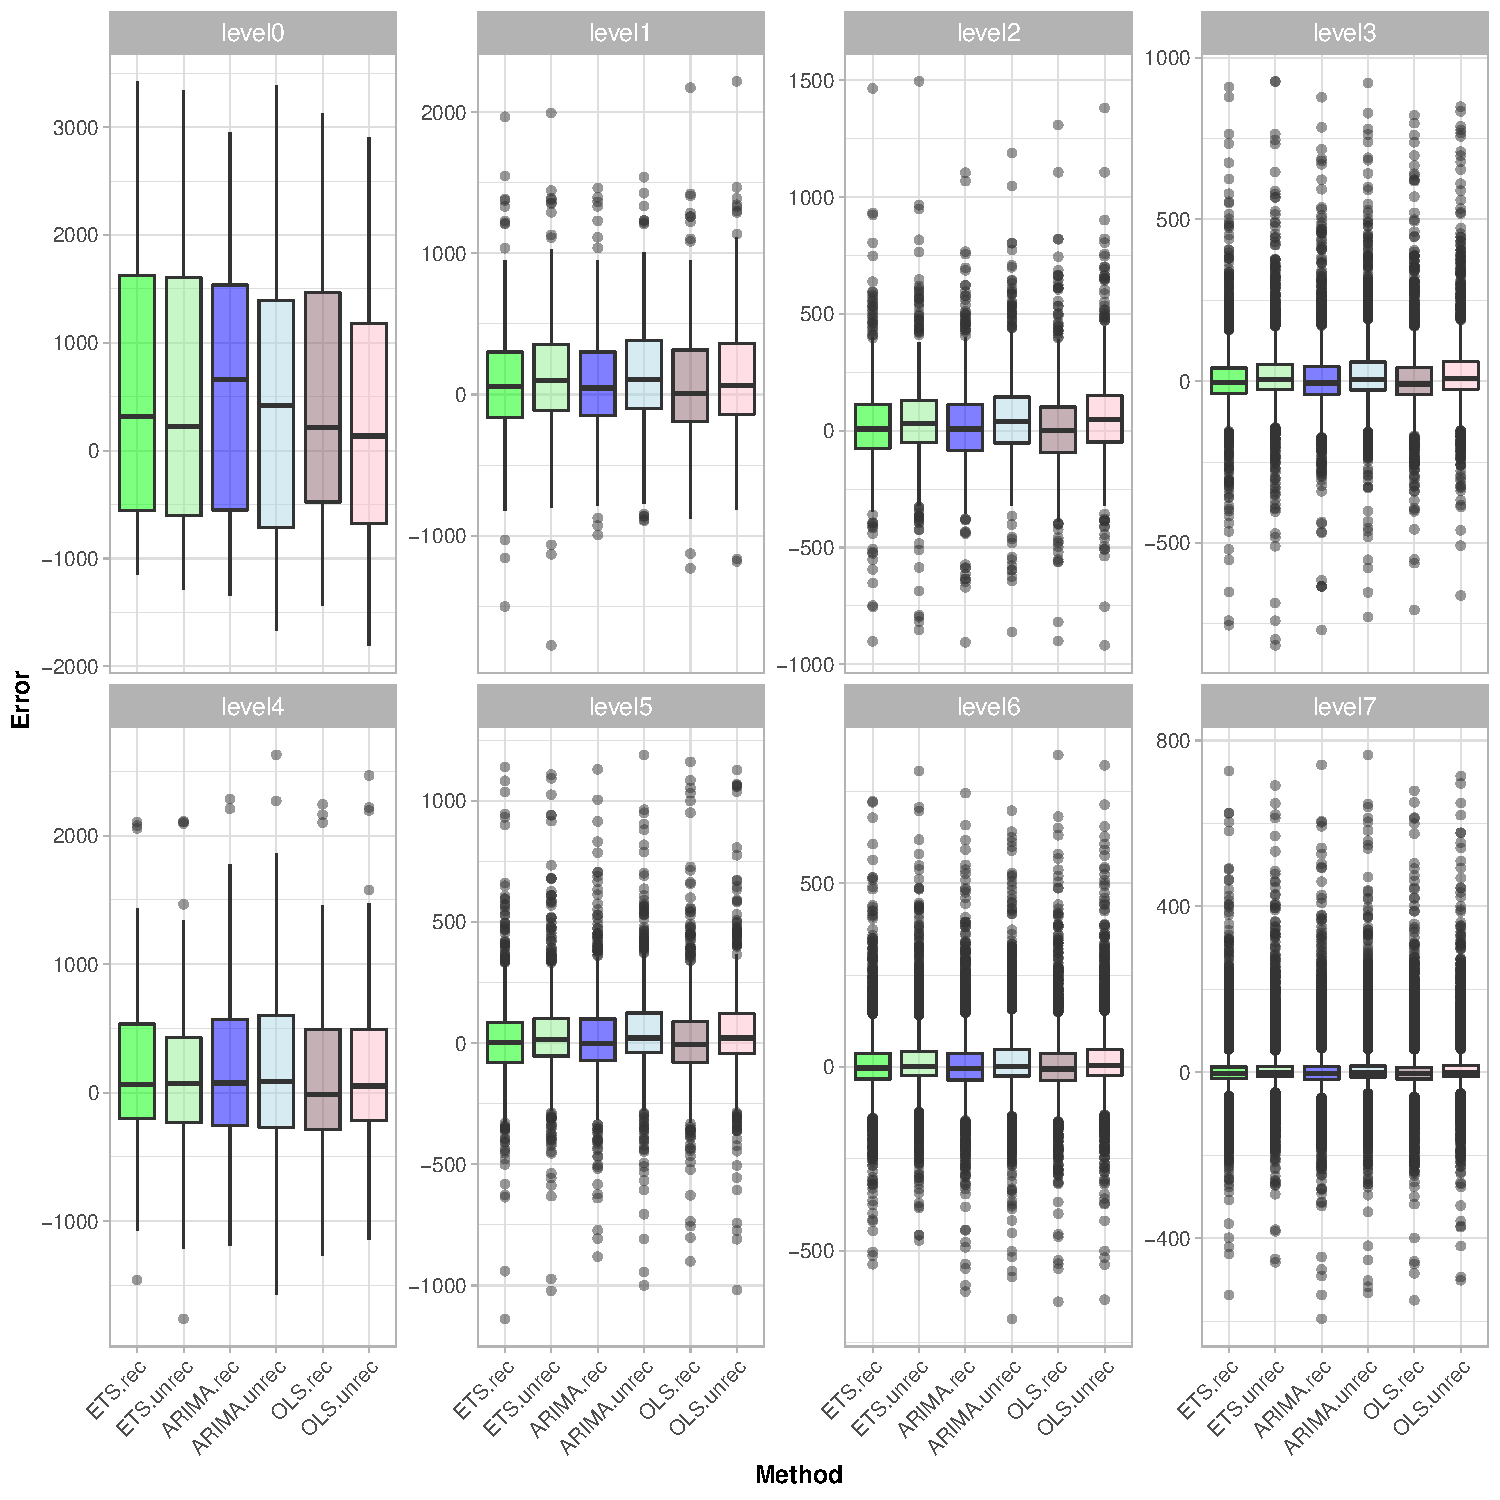
\includegraphics[width=450px,height=300px]{Paper-Figures/results_Tourism/boxplot_1} 

}

\caption{Box plot for forecast errors - Reconciled and unreconciled ETS, ARIMA and OLS in each hierarchy level for 1-step-ahead tourism demand}\label{fig:boxplotrollingtourism}
\end{figure}

\begin{figure}

{\centering 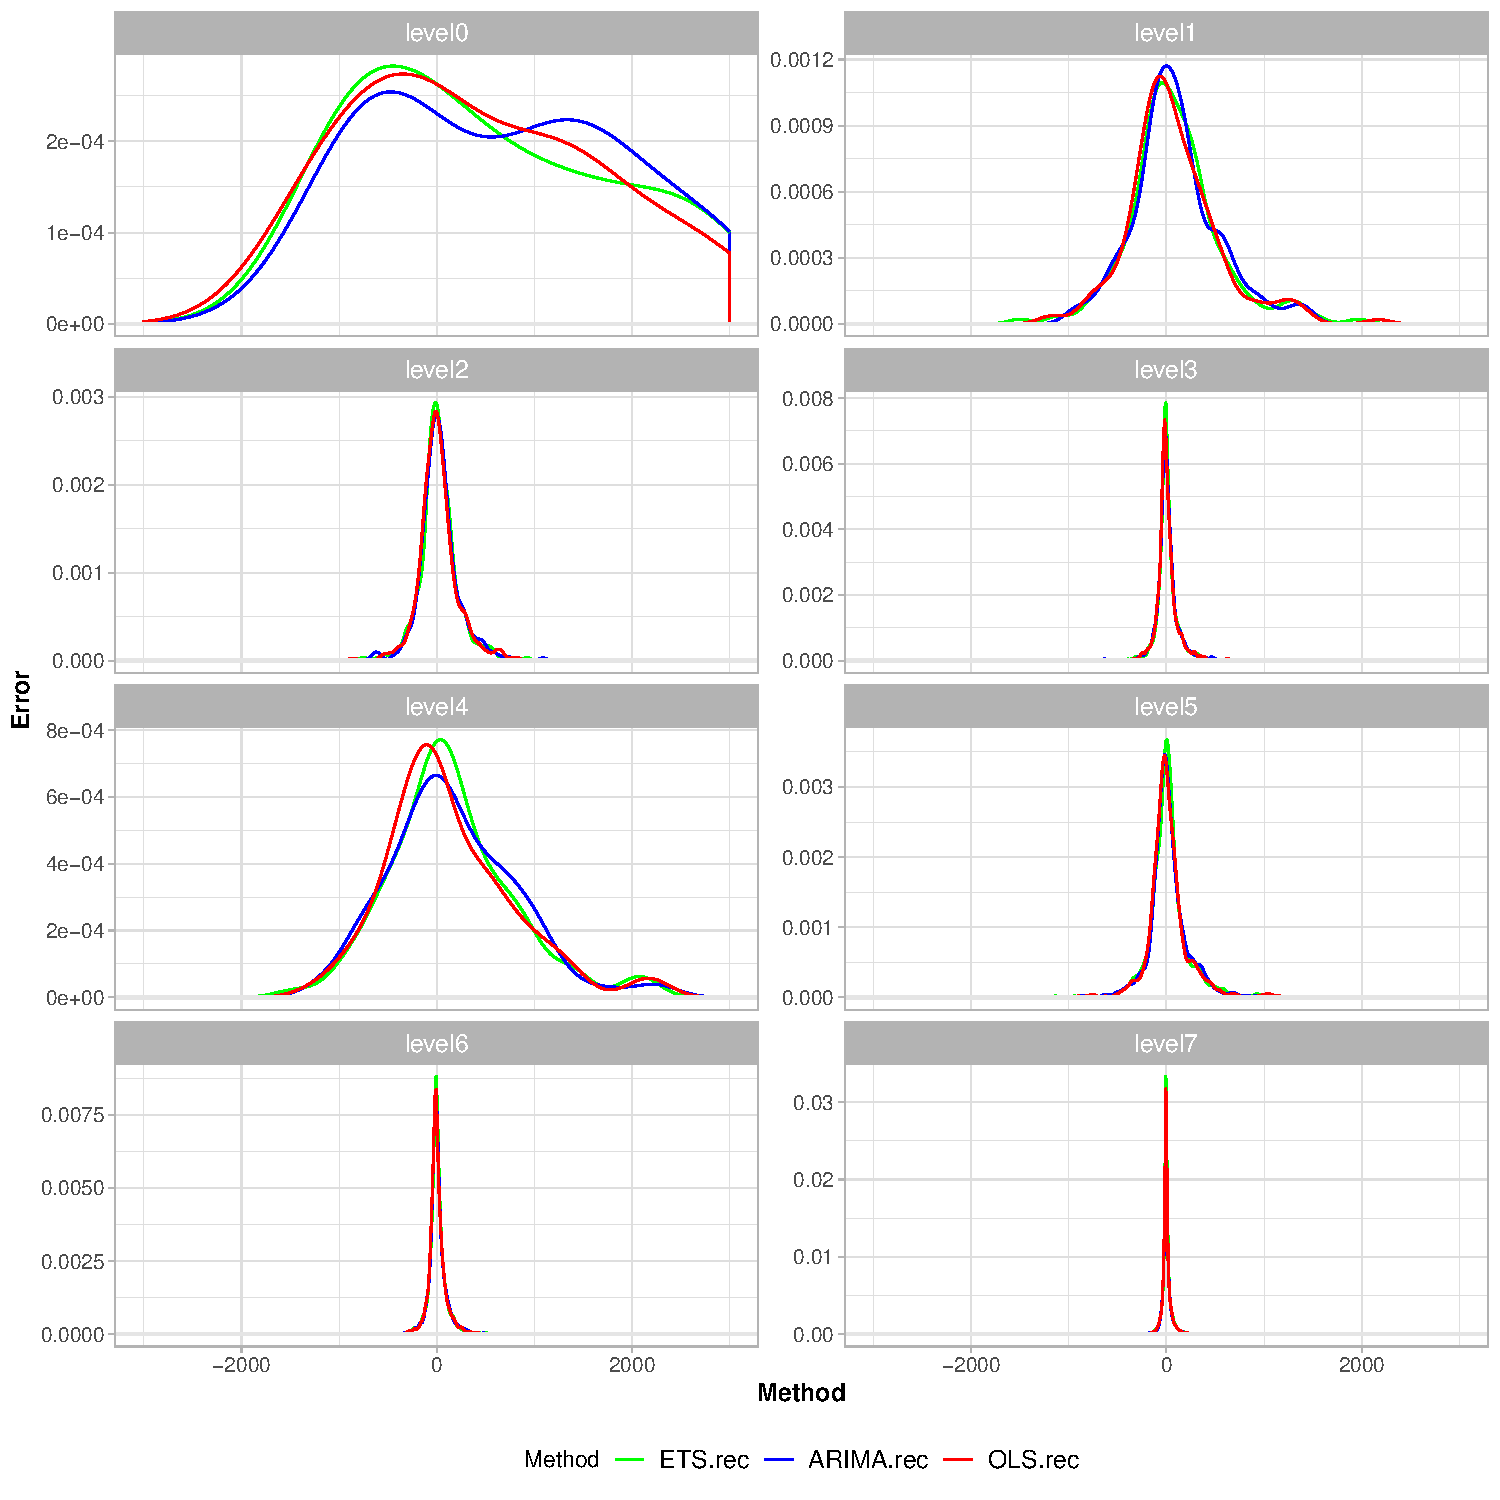
\includegraphics[width=450px,height=550px]{Paper-Figures/results_Tourism/densityplot_1} 

}

\caption{Density plot for forecast errors - Reconciled and unreconciled ETS, ARIMA and OLS in each hierarchy level for 1-step-ahead tourism demand using interval (-1000,3000)}\label{fig:densityplotrollingtourism}
\end{figure}

\begin{table}[t]

\caption{\label{tab:TourismdataresultRMSE}Mean(RMSE) for ETS, ARIMA and OLS with and without reconciliation - 24-step-ahead - Tourism dataset}
\centering
\begin{tabular}{ccccccc}
\toprule
\multicolumn{1}{c}{} & \multicolumn{6}{c}{Mean(RMSE)} \\
\cmidrule(l{2pt}r{2pt}){2-7}
\multicolumn{1}{c}{} & \multicolumn{3}{c}{Unreconciled} & \multicolumn{3}{c}{Reconciled} \\
\cmidrule(l{2pt}r{2pt}){2-4} \cmidrule(l{2pt}r{2pt}){5-7}
 & ETS & ARIMA & OLS & ETS & ARIMA & OLS\\
\midrule
Level 0 & 2238.58 & 3553.99 & 4194.26 & 2250.22 & 3179.39 & 4194.21\\
Level 1 & 593.57 & 570.13 & 827.67 & 553.76 & 626.32 & 827.67\\
Level 2 & 239.52 & 229.64 & 275.99 & 234.21 & 242.46 & 275.99\\
Level 3 & 132.58 & 129.40 & 144.01 & 126.74 & 129.40 & 144.02\\
Level 4 & 766.78 & 824.00 & 1274.00 & 795.48 & 958.24 & 1274.01\\
Level 5 & 226.74 & 241.18 & 285.63 & 222.48 & 236.94 & 285.63\\
Level 6 & 103.02 & 105.38 & 112.20 & 101.95 & 103.93 & 112.19\\
Level 7 & 59.12 & 58.81 & 62.54 & 58.54 & 58.71 & 62.55\\
\bottomrule
\end{tabular}
\end{table}

\begin{figure}

{\centering 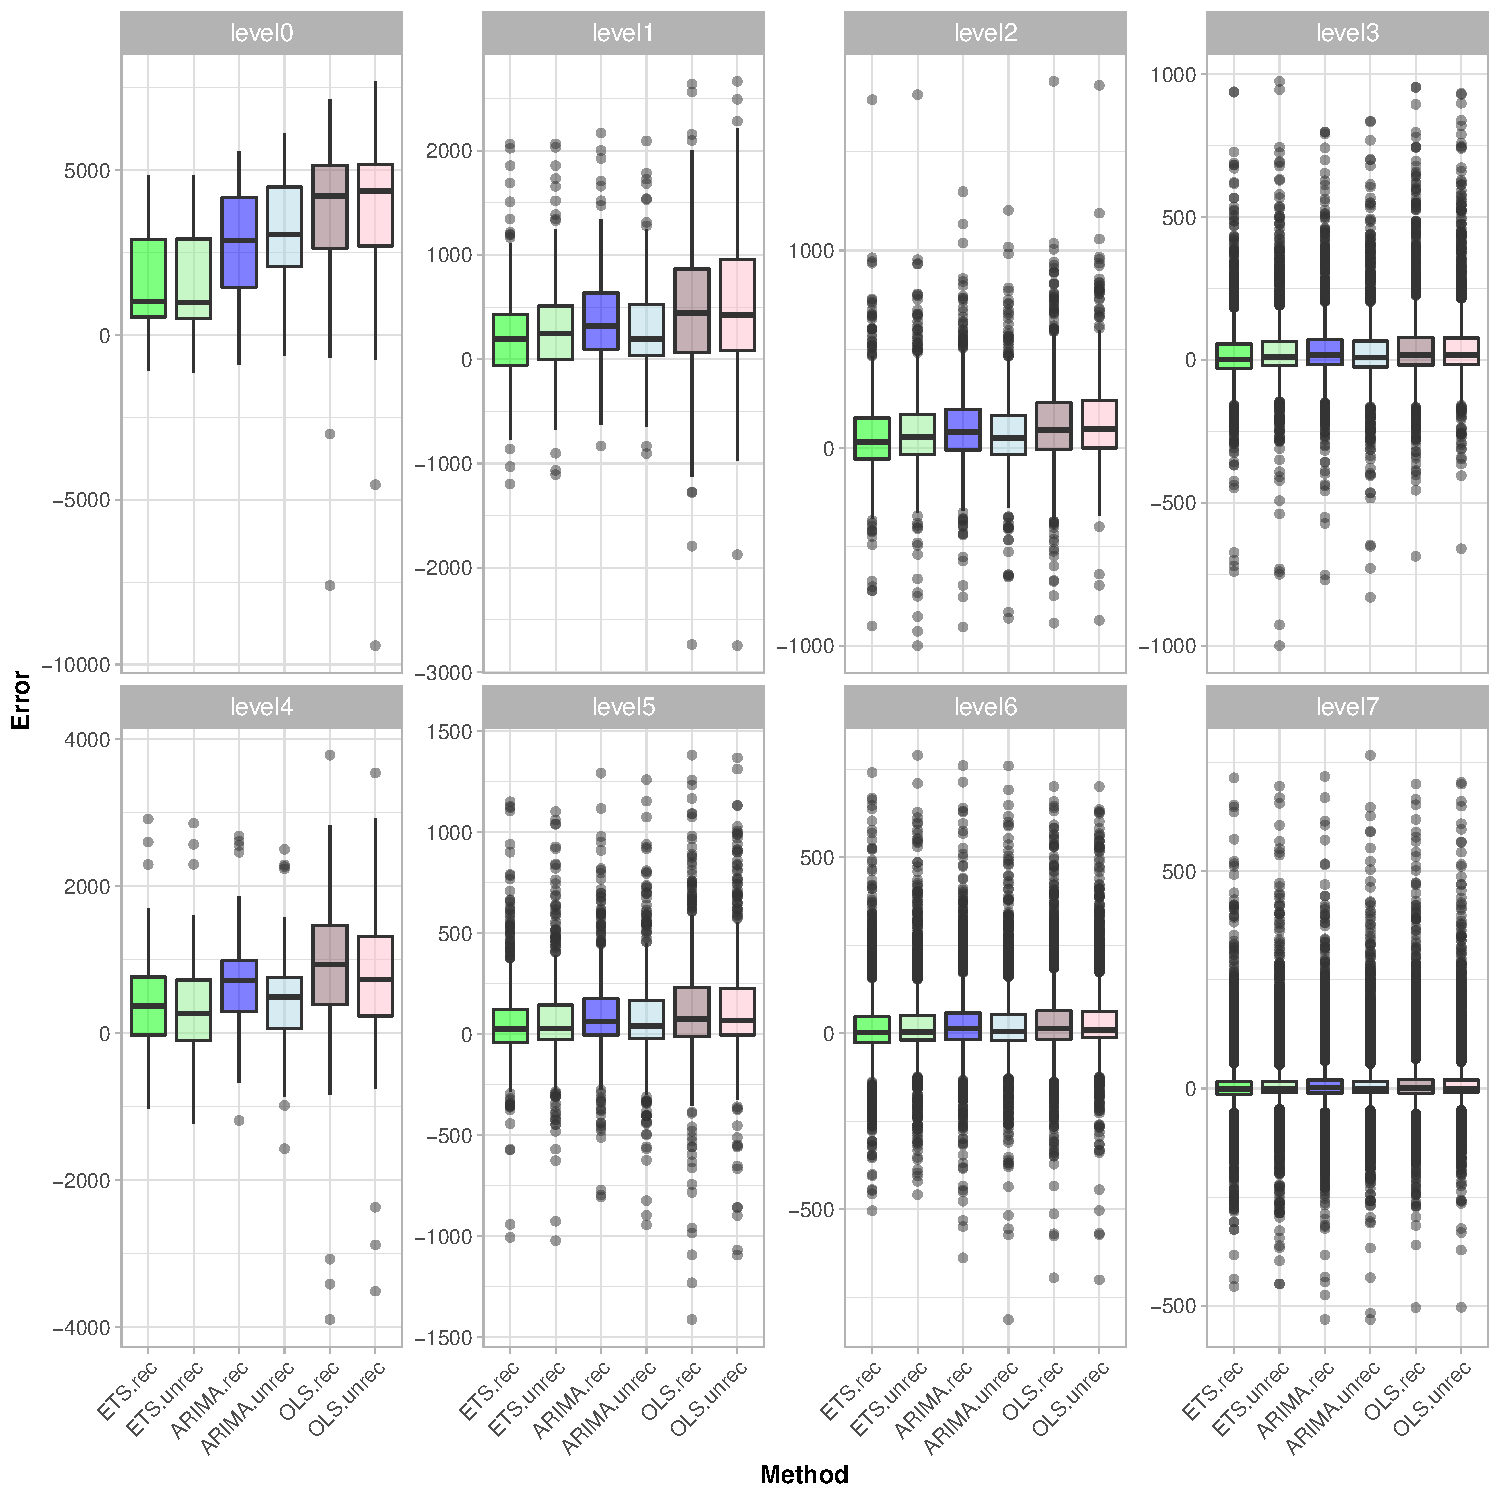
\includegraphics[width=450px,height=300px]{Paper-Figures/results_Tourism/boxplot_24} 

}

\caption{Box plot for forecast errors - Reconciled and unreconciled ETS, ARIMA and OLS in each hierarchy level for 24-step-ahead tourism demand}\label{fig:boxplottourism}
\end{figure}

\begin{figure}

{\centering 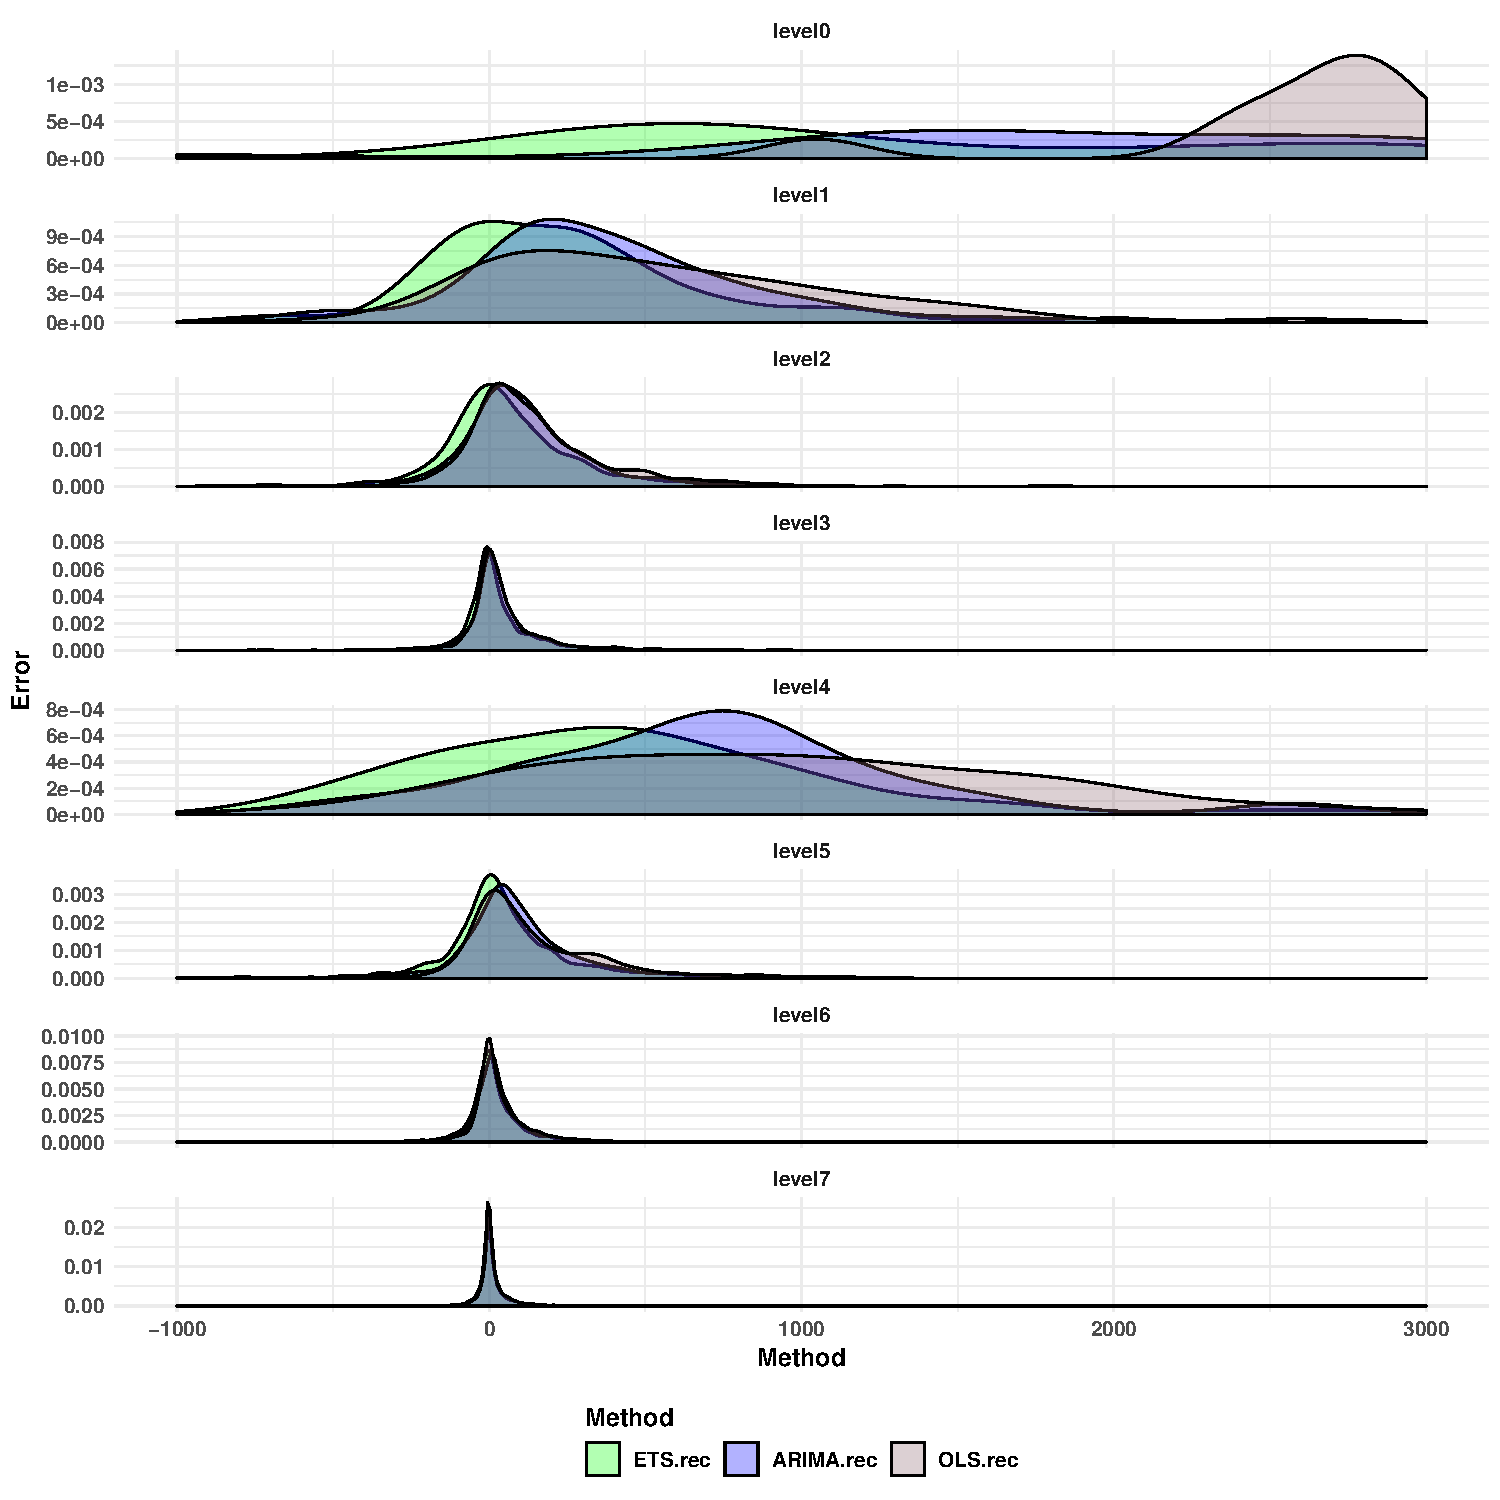
\includegraphics[width=450px,height=550px]{Paper-Figures/results_Tourism/densityplot_24} 

}

\caption{Density plot for forecast errors - Reconciled and unreconciled ETS, ARIMA and OLS in each hierarchy level for 24-step-ahead tourism demand using interval (-1000,3000)}\label{fig:densityplottourism}
\end{figure}

Table \ref{tab:Tourismdatacomputationtime} compares the three methods, computation time for 1-step-ahead and 24-step-ahead forecasting. We see that the OLS forecasting model is much faster compared with the other methods. Also, since reconciliation is a linear process, in all methods, it is very fast and does not affect computation time significantly.

\begin{table}[t]

\caption{\label{tab:Tourismdatacomputationtime}Computation time (seconds) for ETS, ARIMA and OLS with and without reconciliation - 1- and 24-step-ahead - Tourism dataset}
\centering
\begin{tabular}{>{\centering\arraybackslash}p{3cm}>{\centering\arraybackslash}p{3cm}>{\centering\arraybackslash}p{3cm}cc}
\toprule
\multicolumn{1}{c}{} & \multicolumn{4}{c}{Computation time (secs)} \\
\cmidrule(l{2pt}r{2pt}){2-5}
\multicolumn{1}{c}{} & \multicolumn{2}{c}{1-step-ahead} & \multicolumn{2}{c}{24-step-ahead} \\
\cmidrule(l{2pt}r{2pt}){2-3} \cmidrule(l{2pt}r{2pt}){4-5}
 & Unreconciled & Reconciled & Unreconciled & Reconciled\\
\midrule
ETS & 10924.57 & 10924.60 & 407.10 & 407.15\\
ARIMA & 31146.38 & 31146.52 & 1116.15 & 1116.19\\
OLS & 48.40 & 48.31 & 16.66 & 16.85\\
\bottomrule
\end{tabular}
\end{table}

Now since we are using linear model for forecasting, in this part we are including the `easter' information to check its effect on forecasting results. We also add this information on ARIMA models and compare with OLS forecasting model. In Tables \ref{tab:easterroolingRMSE} and \ref{tab:easterRMSE}, we display the average RMSE of ARIMA and OLS including the easter information, ARIMAX and OLSX, across different levels with and without reconciliation. These tables are for 1-step-ahead and 24-step-ahead forecasts. Figure \ref{fig:forecstrolling24tourism} shows the 1-step-ahead and 24-step-ahead forecast results for one of the bottom level series, BACBus (Geelong - Business). In these plots we have both reconciled (solid lines) and unreconciled (dashed lines) forecasts and we see that the reconciliation step improves the forecasts in this series. We also see that the OLS model forecast accuracy is similar to the other two methods. As you can see from the results adding this external data could not change the forecasting results significantly. However in different cases, trying different external data can be helpful in improving the forecasting results.

\begin{table}[t]

\caption{\label{tab:easterroolingRMSE}Mean(RMSE) for ARIMAX and OLSX, adding easter information, with and without reconciliation - 1-step-ahead - Tourism dataset}
\centering
\begin{tabular}{ccccccccc}
\toprule
\multicolumn{1}{c}{} & \multicolumn{8}{c}{Mean(RMSE)} \\
\cmidrule(l{2pt}r{2pt}){2-9}
\multicolumn{1}{c}{} & \multicolumn{4}{c}{Unreconciled} & \multicolumn{4}{c}{Reconciled} \\
\cmidrule(l{2pt}r{2pt}){2-5} \cmidrule(l{2pt}r{2pt}){6-9}
 & ARIMA & OLS & ARIMAX & OLSX & ARIMA & OLS & ARIMAX & OLSX\\
\midrule
Level 0 & 1445.49 & 1415.06 & 1564.95 & 1444.49 & 1453.44 & 1454.39 & 1546.53 & 1487.23\\
Level 1 & 493.14 & 510.83 & 500.66 & 514.29 & 457.65 & 488.33 & 472.03 & 492.68\\
Level 2 & 219.01 & 224.50 & 220.91 & 225.82 & 207.52 & 212.44 & 210.47 & 213.48\\
Level 3 & 125.08 & 123.97 & 125.85 & 123.69 & 120.52 & 119.52 & 121.02 & 119.44\\
Level 4 & 709.22 & 694.50 & 702.78 & 680.56 & 679.74 & 678.54 & 682.92 & 662.45\\
Level 5 & 220.08 & 216.11 & 222.07 & 215.15 & 209.39 & 211.13 & 211.45 & 209.55\\
Level 6 & 102.41 & 101.03 & 103.04 & 100.93 & 99.77 & 98.56 & 100.53 & 98.49\\
Level 7 & 58.20 & 58.17 & 58.60 & 58.05 & 57.68 & 57.20 & 58.04 & 57.15\\
\bottomrule
\end{tabular}
\end{table}

\begin{table}[t]

\caption{\label{tab:easterRMSE}Mean(RMSE) for ARIMAX and OLSX, adding easter information, with and without reconciliation - 24-step-ahead - Tourism dataset}
\centering
\begin{tabular}{ccccccccc}
\toprule
\multicolumn{1}{c}{} & \multicolumn{8}{c}{Mean(RMSE)} \\
\cmidrule(l{2pt}r{2pt}){2-9}
\multicolumn{1}{c}{} & \multicolumn{4}{c}{Unreconciled} & \multicolumn{4}{c}{Reconciled} \\
\cmidrule(l{2pt}r{2pt}){2-5} \cmidrule(l{2pt}r{2pt}){6-9}
 & ARIMA & OLS & ARIMAX & OLSX & ARIMA & OLS & ARIMAX & OLSX\\
\midrule
Level 0 & 3553.99 & 4194.26 & 3528.13 & 4215.36 & 3179.39 & 4194.21 & 3114.40 & 4215.28\\
Level 1 & 570.13 & 827.67 & 509.84 & 828.10 & 626.32 & 827.67 & 603.66 & 828.09\\
Level 2 & 229.64 & 275.99 & 235.06 & 276.75 & 242.46 & 275.99 & 243.76 & 276.75\\
Level 3 & 129.40 & 144.01 & 129.39 & 144.86 & 129.40 & 144.02 & 129.63 & 144.86\\
Level 4 & 824.00 & 1274.00 & 811.08 & 1292.03 & 958.24 & 1274.01 & 930.72 & 1292.03\\
Level 5 & 241.18 & 285.63 & 232.88 & 289.12 & 236.94 & 285.63 & 229.59 & 289.12\\
Level 6 & 105.38 & 112.20 & 104.73 & 113.01 & 103.93 & 112.19 & 104.50 & 113.00\\
Level 7 & 58.81 & 62.54 & 59.22 & 62.97 & 58.71 & 62.55 & 59.02 & 62.99\\
\bottomrule
\end{tabular}
\end{table}

\begin{figure}

{\centering 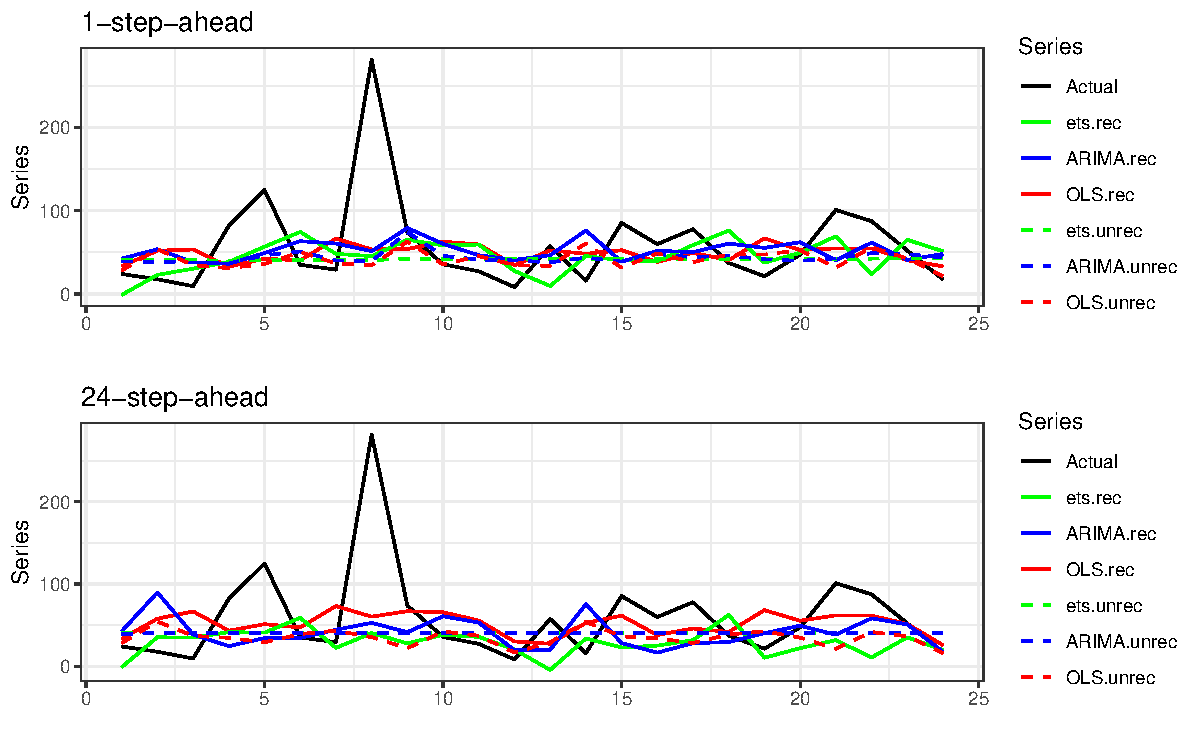
\includegraphics[width=450px,height=300px]{hcf_files/figure-latex/forecstrolling24tourism-1} 

}

\caption{Comparing Actual test set, Reconciled and unreconciled ETS, ARIMA and OLS for BACBus bottom level series for 1-step-ahead and 24-step-ahead tourism demand}\label{fig:forecstrolling24tourism}
\end{figure}

\hypertarget{wikipedia-pageviews}{%
\subsection{Wikipedia pageviews}\label{wikipedia-pageviews}}

The second dataset consists of one year of daily data (2016-06-01 to 2017-06-29) on Wikipedia pageviews for the most popular social networks articles \autocite{ashouri2018}. This dataset is noisier compared with the Australian monthly tourism data and forecasting its series is more challenging. It has a grouped structure, with grouping attributes: `Agent': Spider, User, `Access': Desktop, Mobile app, Mobile web, `Language': en (English), de (German), es (Spanish), zh (Chinese) and `Purpose': Blogging related, Business, Gaming, General purpose, Life style, Photo sharing, Reunion, Travel, Video (check Table \ref{tab:wikipediagroupingstructure}). We display the group structure in Table \ref{tab:wikipediagroupingstructure} and Figure \ref{fig:wikigroupstructure}. In Figure \ref{fig:wikigroupstructure} we use one possible hierarchy for this dataset, but the order of the hierarchy can be switched.
The final dataset includes 913 time series, each with length 394. The group structure and different levels include:

\begin{itemize}
\tightlist
\item
  Level 0 = Total
\item
  Level 1 = Agent
\item
  Level 2 = Access
\item
  Level 3 = Language
\item
  Level 4 = Purpose
\item
  Level 5 = bottom level series
\end{itemize}

For this daily dataset, in the OLS forecasting model we include in the predictor matrix a linear trend, 6 seasonal dummies and 7 lags. We partitioned the data into two parts training and test sets. We used the last 28 days for our test set and the rest for the training set.

\begin{table}[t]

\caption{\label{tab:wikipediagroupingstructure}Social networking Wikipedia article grouping structure}
\centering
\begin{tabular}{crcr}
\toprule
Series & Name & Series & Name\\
\midrule
Total &  & Language & \\
1 & Social Network & 10 & zh (Chinese)\\
Agent &  & Purpose & \\
2 & Spider & 11 & Blogging related\\
3 & User & 12 & Business\\
Access &  & 13 & Gaming\\
4 & Desktop & 14 & General purpose\\
5 & Mobile app & 15 & Life style\\
6 & Mobile web & 16 & Photo sharing\\
Language &  & 17 & Reunion\\
7 & en (English) & 18 & Travel\\
8 & de (German) & 19 & Video\\
9 & es (Spanish) &  & \\
\bottomrule
\end{tabular}
\end{table}

\begin{figure}

{\centering 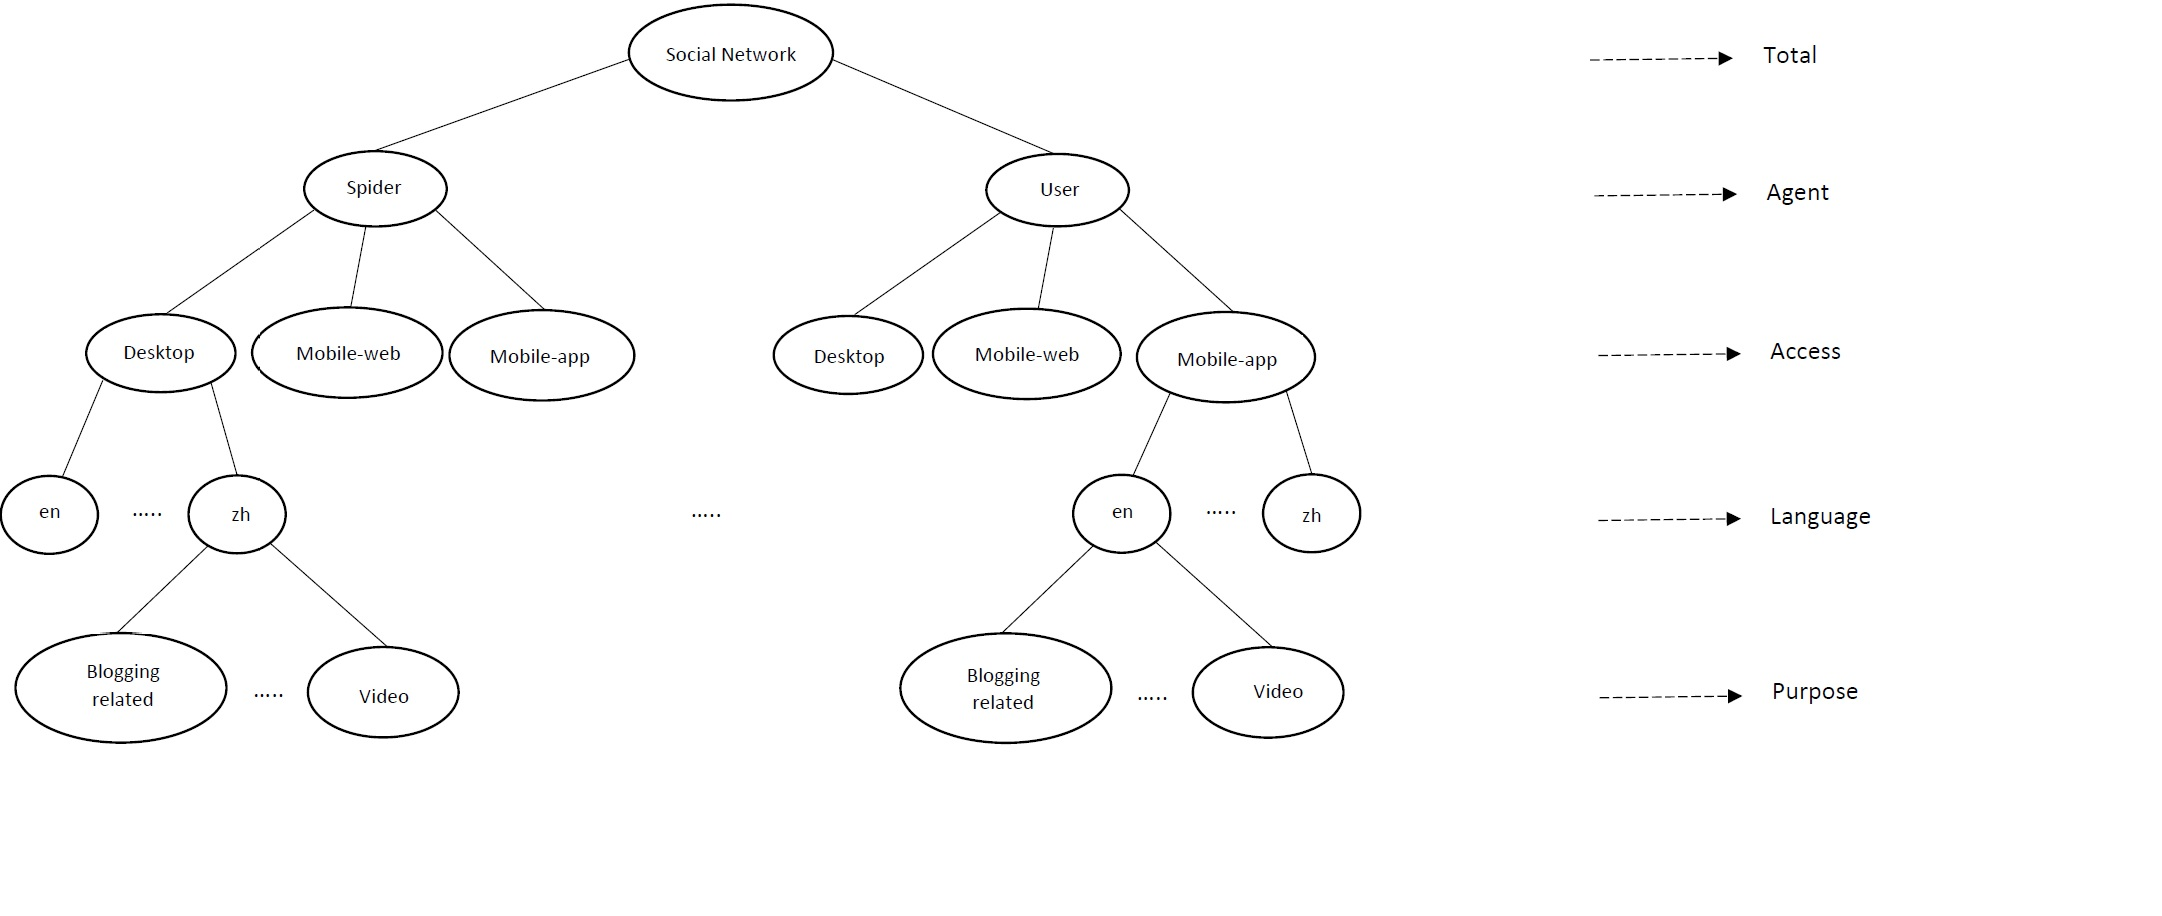
\includegraphics[width=500px,height=250px]{Paper-Figures/Wiki_group_structure} 

}

\caption{One of the possible hierarchy structures for Wikipedia pageview dataset}\label{fig:wikigroupstructure}
\end{figure}

Table \ref{tab:wikipediadataresulrolling}, \ref{tab:wikipediadataresultRMSE} and \ref{tab:wikipediadatacomputationtime} represent the RMSE results and computation time. Although these time series are noisier, still we get acceptable results for the OLS forecasting model compared with ETS and ARIMA. In this case, we get similar results with and without the reconciliation step in the forecasted errors.

Figures \ref{fig:boxplotrollingwiki} and \ref{fig:boxplotwiki} display the forecast error box plot. These plots are for 1-step-ahead and 28-step-ahead forecasts in each level of grouping. Further, we can see that the error distribution is almost similar in all levels across the different methods. The only exception is the Total series, where ETS performs significantly better than ARIMA and OLS. We also note that the reconciliation is less effective.

Figures \ref{fig:densityplotrollingwiki} and \ref{fig:densityplotwiki} show the density plots for the forecast errors. For both 1-step-ahead and 28-step-ahead forecasts, we can see the density structure of the forecast errors across ETS, ARIMA and the OLS forecasting model. Except for the Total series which ETS works better, in all the other levels are the models have similar structure for the forecast errors.

\begin{table}[t]

\caption{\label{tab:wikipediadataresulrolling}Mean(RMSE) for ETS, ARIMA and OLS with and without reconciliation - 1-step-ahead - Wikipedia dataset}
\centering
\begin{tabular}{ccccccc}
\toprule
\multicolumn{1}{c}{} & \multicolumn{6}{c}{Mean(RMSE)} \\
\cmidrule(l{2pt}r{2pt}){2-7}
\multicolumn{1}{c}{} & \multicolumn{3}{c}{Unreconciled} & \multicolumn{3}{c}{Reconciled} \\
\cmidrule(l{2pt}r{2pt}){2-4} \cmidrule(l{2pt}r{2pt}){5-7}
 & ETS & ARIMA & OLS & ETS & ARIMA & OLS\\
\midrule
Level 0 & 10773.66 & 15060.65 & 15748.18 & 11014.73 & 14276.47 & 15270.23\\
Level 1 & 8272.92 & 10196.34 & 10623.85 & 7736.88 & 9904.12 & 10673.98\\
Level 2 & 6524.72 & 6705.03 & 6979.58 & 6257.44 & 7142.49 & 7285.97\\
Level 3 & 4870.08 & 6333.02 & 7150.13 & 4981.91 & 6369.98 & 7106.11\\
Level 4 & 5233.50 & 4659.53 & 4675.18 & 5001.40 & 4586.53 & 4650.26\\
Level 5 & 358.90 & 238.97 & 254.98 & 362.25 & 241.60 & 256.11\\
\bottomrule
\end{tabular}
\end{table}

\begin{figure}

{\centering 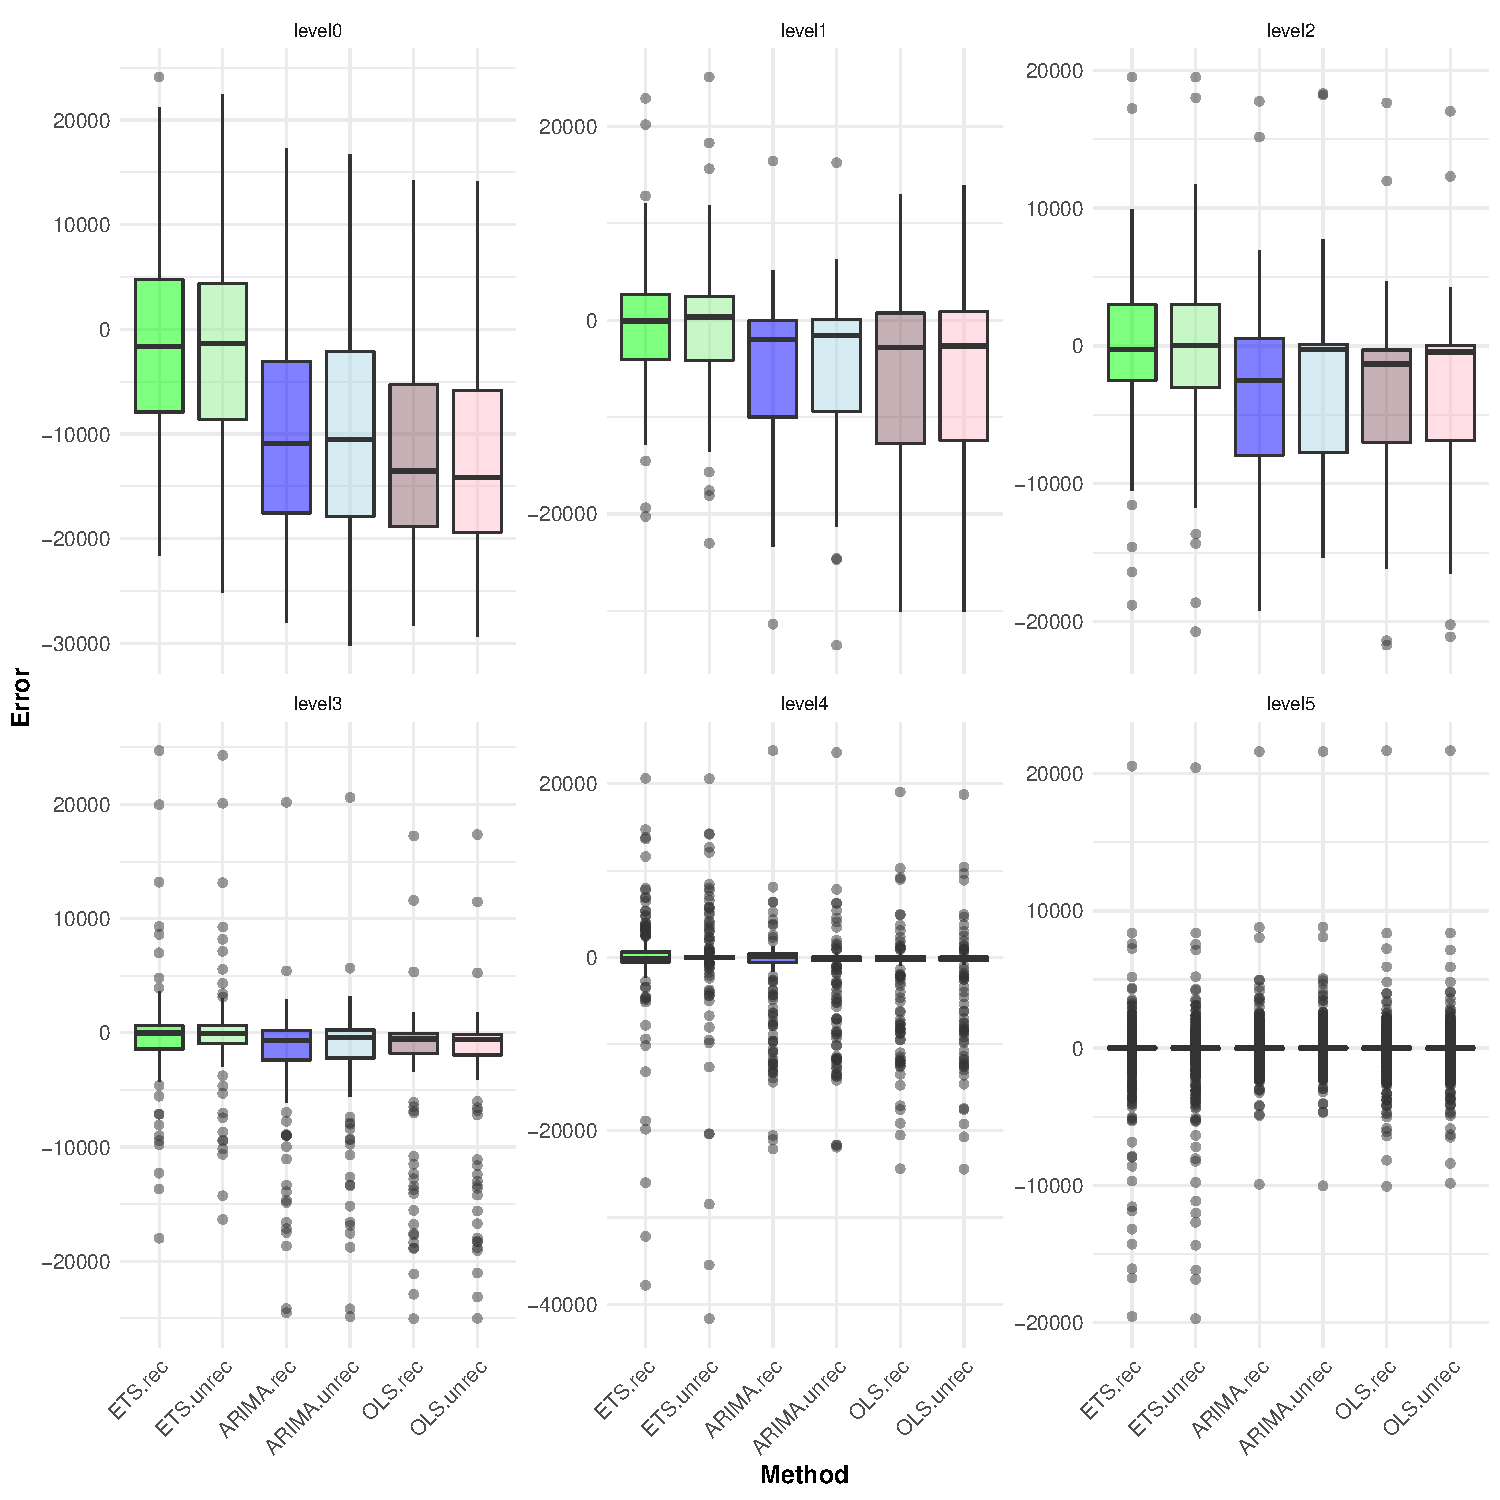
\includegraphics[width=450px,height=300px]{Paper-Figures/results_Wikipedia/boxplot_1} 

}

\caption{Box plot for forecast errors -  Reconciled and unreconciled ETS, ARIMA and OLS in each hierarchy level for 1-step-ahead Wikipedia pageviews}\label{fig:boxplotrollingwiki}
\end{figure}

\begin{figure}

{\centering 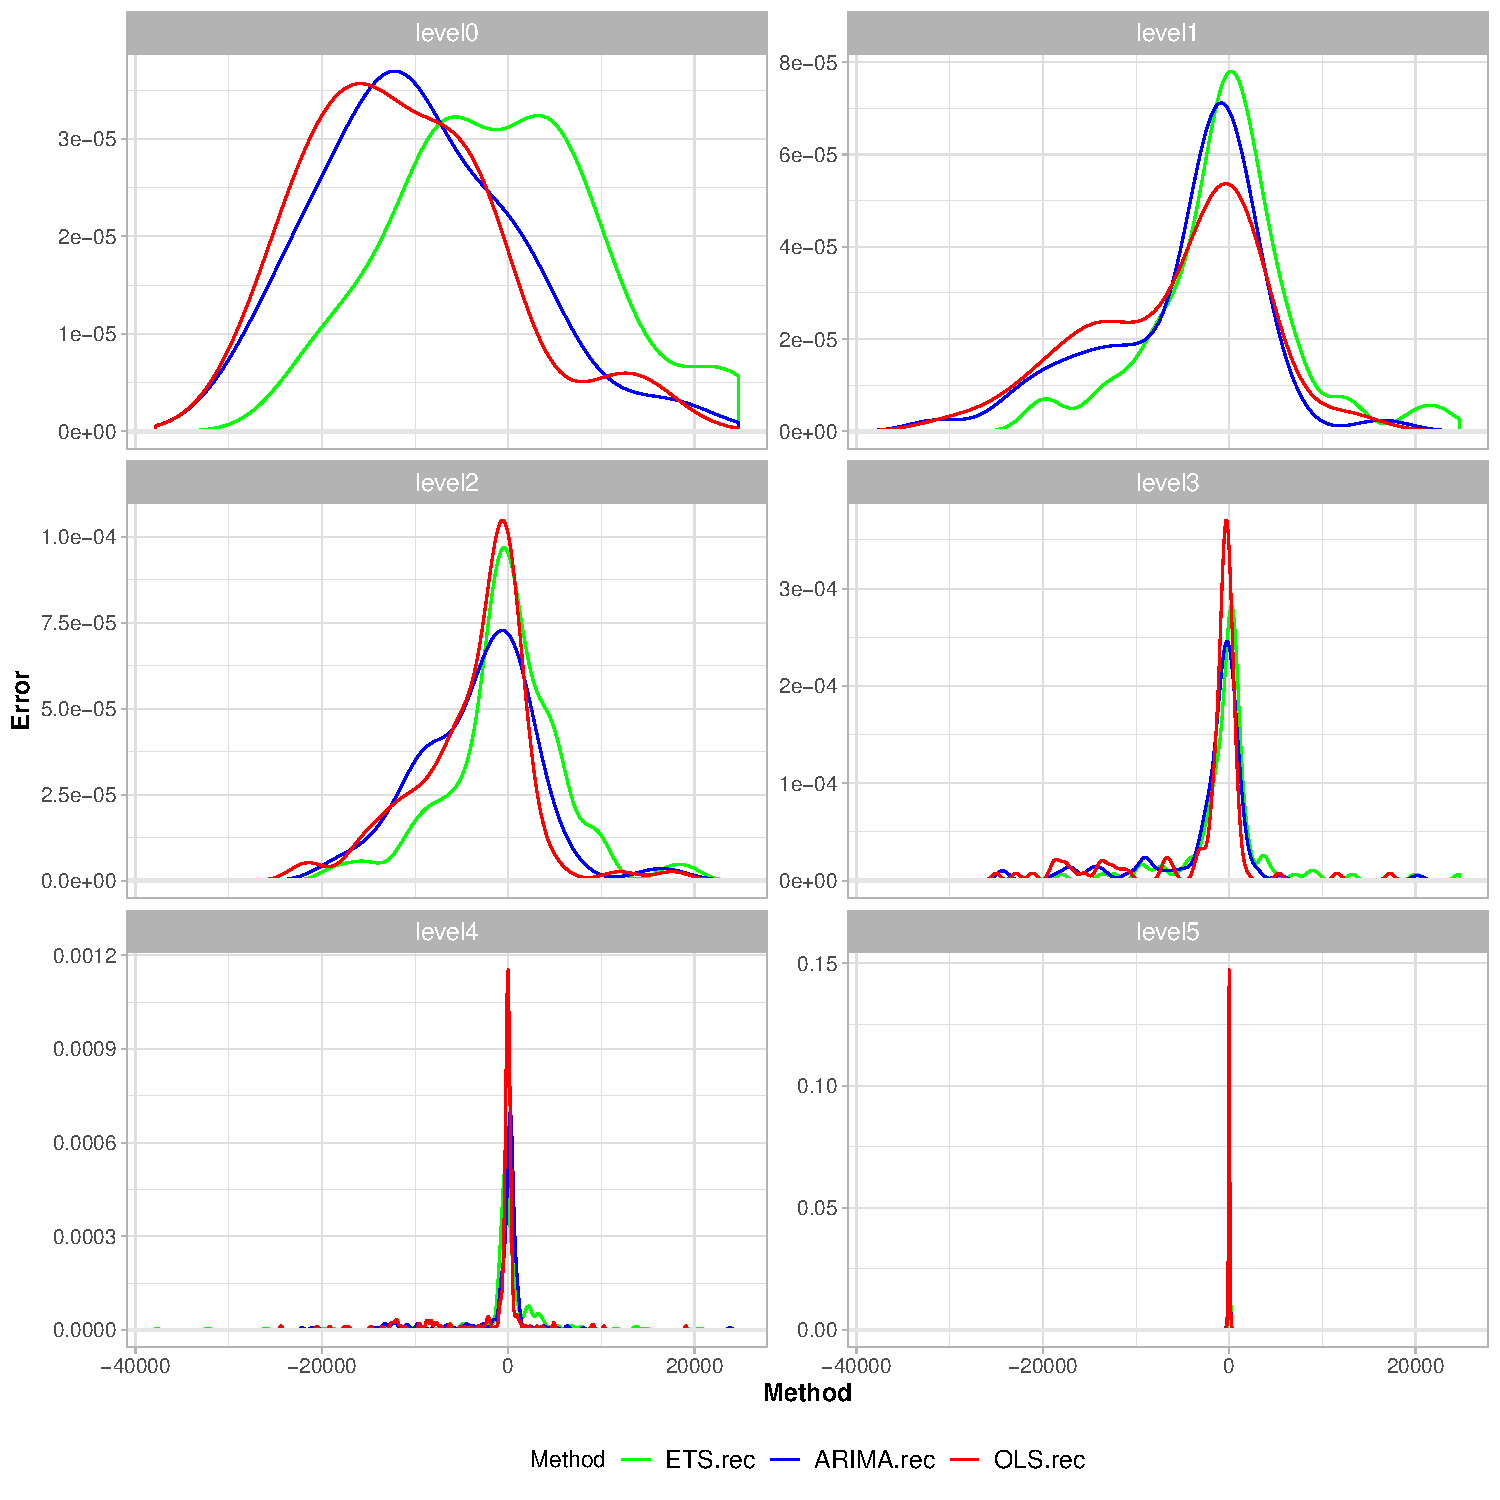
\includegraphics[width=450px,height=550px]{Paper-Figures/results_Wikipedia/densityplot_1} 

}

\caption{Density plot for forecast errors -  Reconciled and unreconciled ETS, ARIMA and OLS in each hierarchy level for 1-step-ahead Wikipedia pageviews}\label{fig:densityplotrollingwiki}
\end{figure}

\begin{table}[t]

\caption{\label{tab:wikipediadataresultRMSE}Mean(RMSE) for ETS, ARIMA and OLS with and without reconciliation - 28-step-ahead - Wikipedia dataset}
\centering
\begin{tabular}{ccccccc}
\toprule
\multicolumn{1}{c}{} & \multicolumn{6}{c}{Mean(RMSE)} \\
\cmidrule(l{2pt}r{2pt}){2-7}
\multicolumn{1}{c}{} & \multicolumn{3}{c}{Unreconciled} & \multicolumn{3}{c}{Reconciled} \\
\cmidrule(l{2pt}r{2pt}){2-4} \cmidrule(l{2pt}r{2pt}){5-7}
 & ETS & ARIMA & OLS & ETS & ARIMA & OLS\\
\midrule
Level 0 & 14846.93 & 24298.84 & 29840.58 & 14999.18 & 24649.91 & 29665.70\\
Level 1 & 13608.73 & 17277.01 & 21165.30 & 12240.30 & 16810.45 & 21048.06\\
Level 2 & 7117.43 & 10731.97 & 12678.89 & 7523.43 & 11068.81 & 12811.18\\
Level 3 & 6475.90 & 9580.38 & 12056.62 & 6509.03 & 9799.11 & 12112.46\\
Level 4 & 5302.74 & 8611.25 & 8451.09 & 5307.34 & 8239.77 & 8460.35\\
Level 5 & 435.64 & 390.05 & 389.41 & 437.67 & 391.22 & 390.97\\
\bottomrule
\end{tabular}
\end{table}

\begin{figure}

{\centering 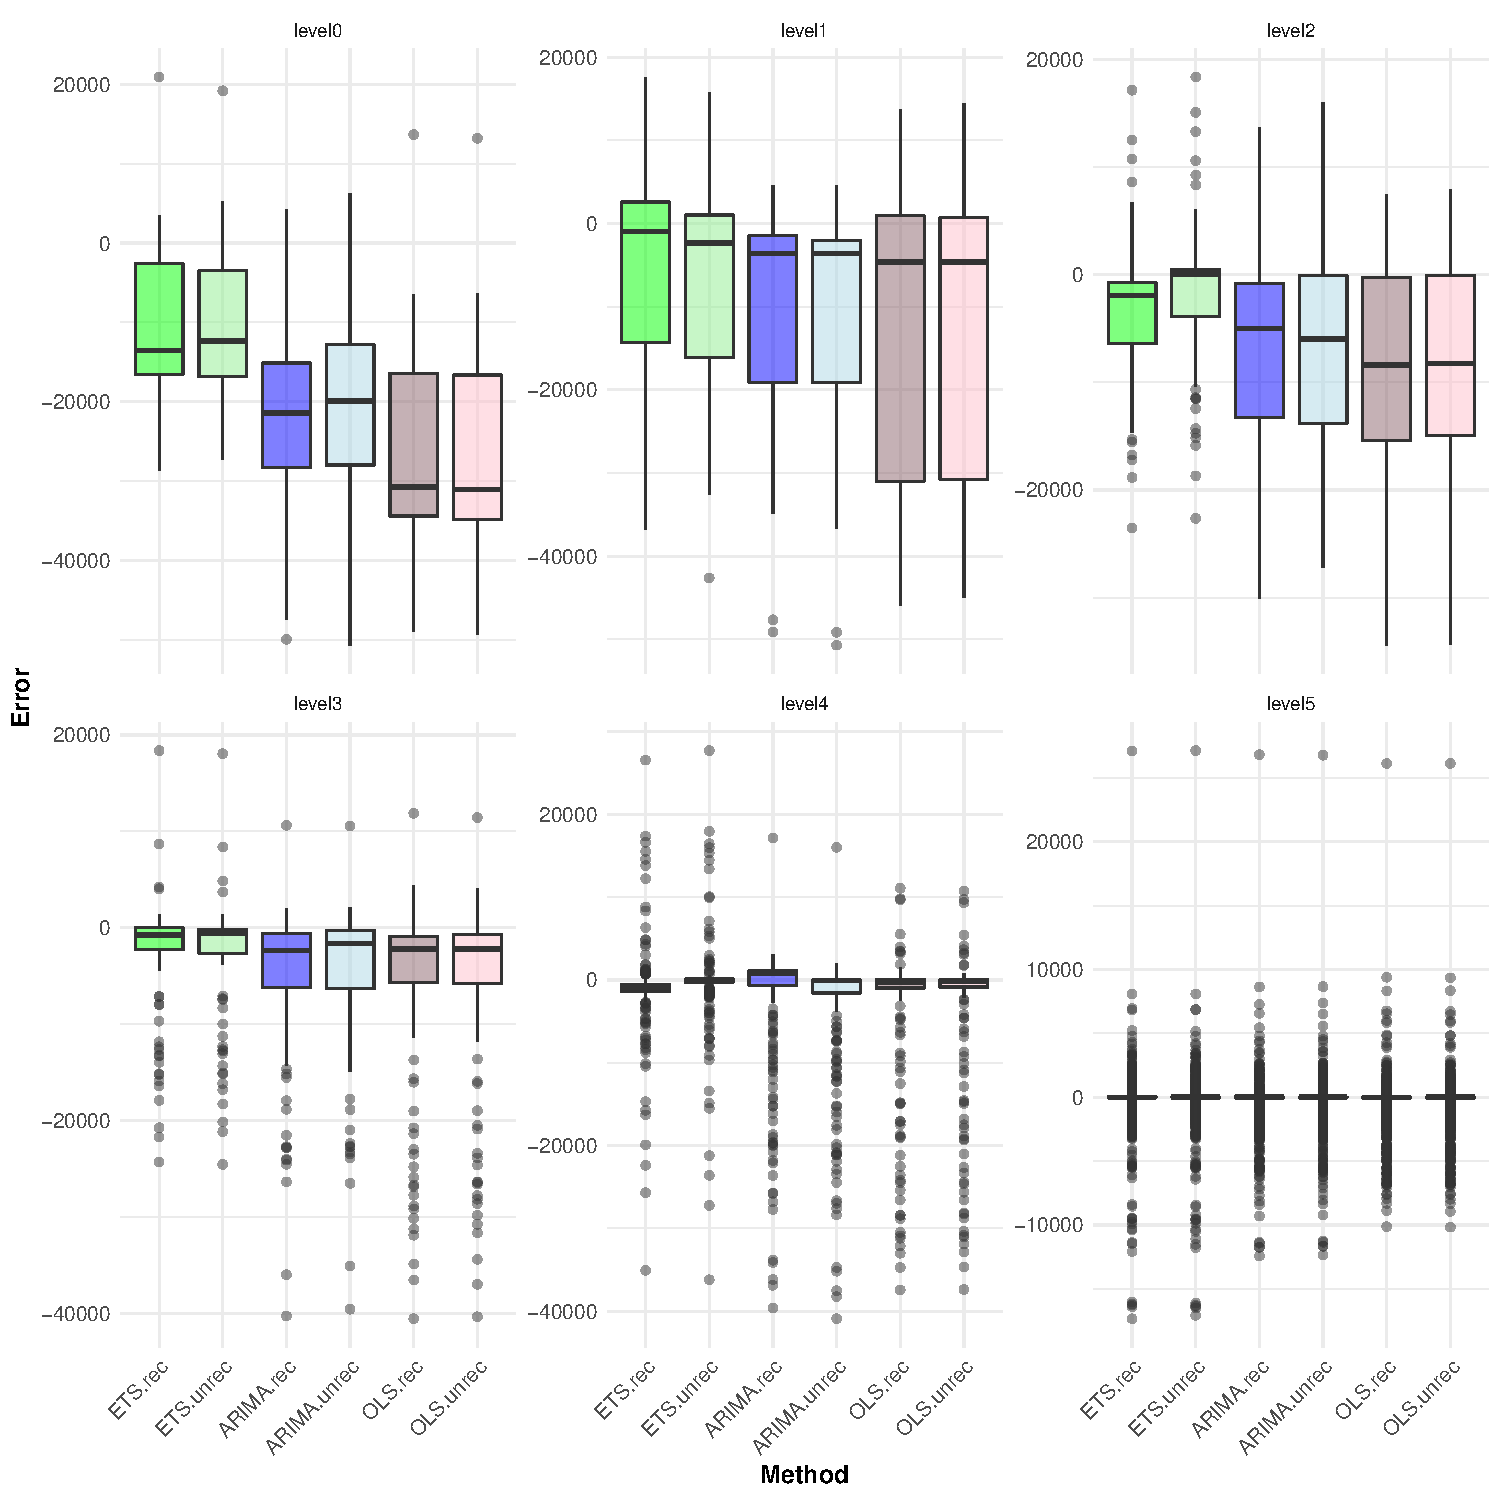
\includegraphics[width=450px,height=300px]{Paper-Figures/results_Wikipedia/boxplot_28} 

}

\caption{Box plot for forecast errors -  Reconciled and unreconciled ETS, ARIMA and OLS in each hierarchy level for 28-step-ahead Wikipedia pageviews}\label{fig:boxplotwiki}
\end{figure}

\begin{figure}

{\centering 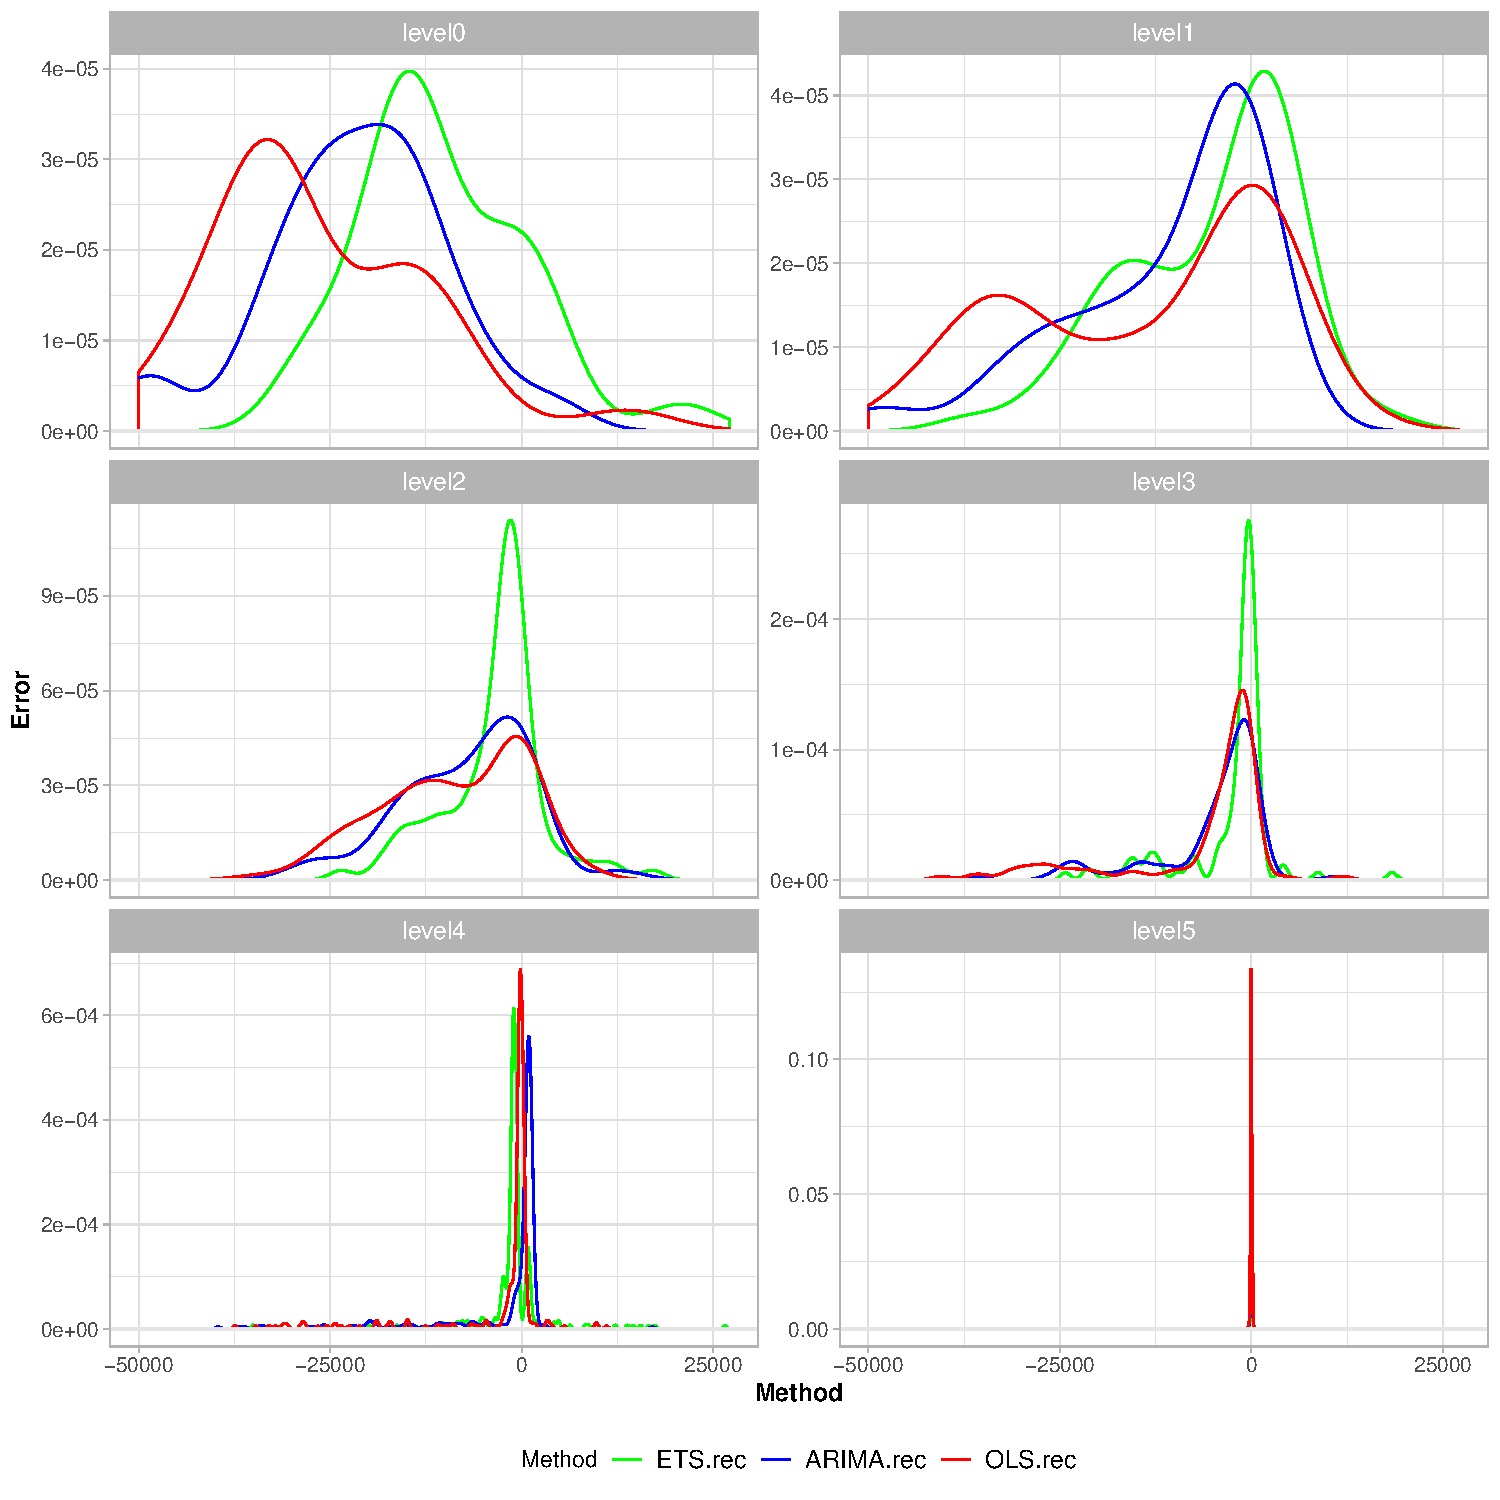
\includegraphics[width=450px,height=550px]{Paper-Figures/results_Wikipedia/densityplot_28} 

}

\caption{Density plot for forecast errors -  Reconciled and unreconciled ETS, ARIMA and OLS in each hierarchy level for 28-step-ahead Wikipedia pageviews}\label{fig:densityplotwiki}
\end{figure}

In Figure \ref{fig:forecstrolling28wiki}, we display results for one of the bottom level series, desktopusenPho (desktop-user-english-photo sharing). The plot shows 1-step-ahead and 28-step-ahead forecast results for ETS, ARIMA and OLS, with (solid lines) and without (dashed lines) applying reconciliation. We see that the OLS forecasting model performs close to the other two methods, and reconciliation improves the forecasts.

\begin{figure}

{\centering 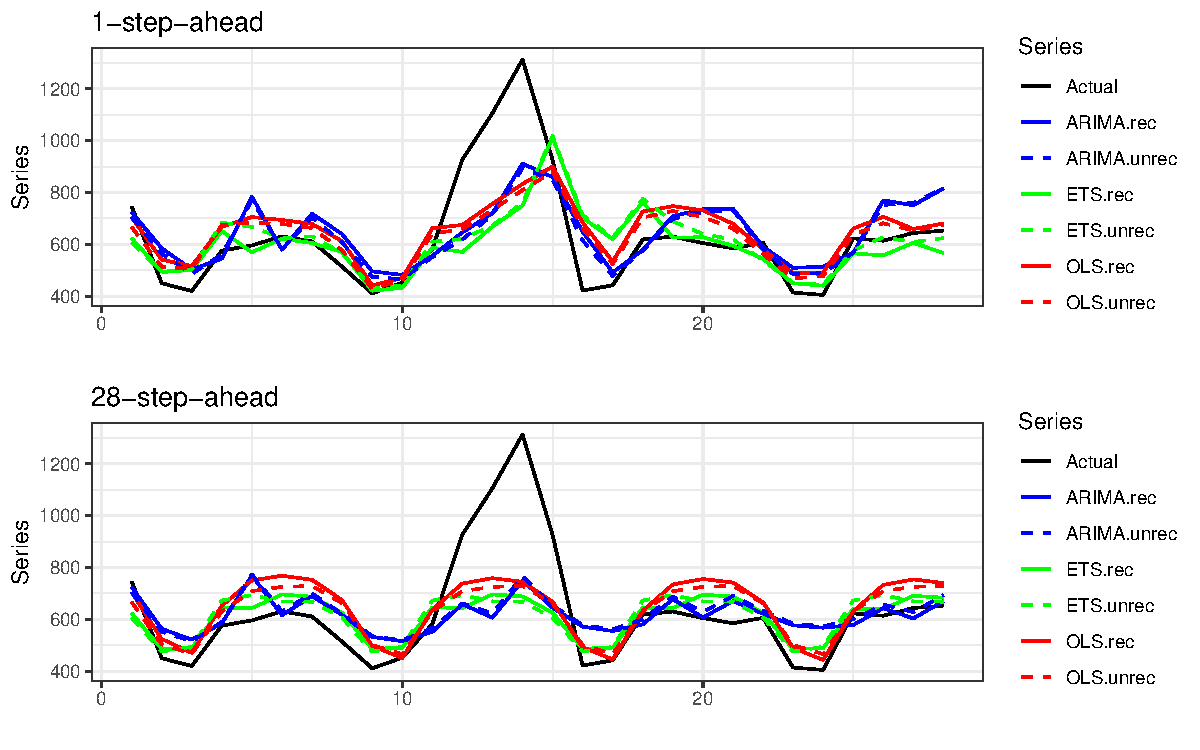
\includegraphics[width=400px,height=300px]{hcf_files/figure-latex/forecstrolling28wiki-1} 

}

\caption{Comparing Actual test set, Reconciled and unreconciled ETS, ARIMA and OLS for desktopusenPho (desktop-user-english-photo sharing)  bottom level series- 1- and 28-step-ahead Wikipedia pageviews}\label{fig:forecstrolling28wiki}
\end{figure}

Lastly, Table \ref{tab:wikipediadatacomputationtime} presents the computation times for all three methods. ETS and ARIMA are clearly much more computationally heavy compared with OLS. As in the Australian tourism dataset, running reconciliation does not have much effect on computation time.

\begin{table}[t]

\caption{\label{tab:wikipediadatacomputationtime}Computation time (seconds) for ETS, ARIMA and OLS with and without reconciliation - 1- and 28-step-ahead - Wikipedia dataset}
\centering
\begin{tabular}{>{\centering\arraybackslash}p{3cm}>{\centering\arraybackslash}p{3cm}>{\centering\arraybackslash}p{3cm}cc}
\toprule
\multicolumn{1}{c}{} & \multicolumn{4}{c}{Computation time (secs)} \\
\cmidrule(l{2pt}r{2pt}){2-5}
\multicolumn{1}{c}{} & \multicolumn{2}{c}{1-step-ahead} & \multicolumn{2}{c}{28-step-ahead} \\
\cmidrule(l{2pt}r{2pt}){2-3} \cmidrule(l{2pt}r{2pt}){4-5}
 & Unreconciled & Reconciled & Unreconciled & Reconciled\\
\midrule
ETS & 13963.93 & 13963.96 & 450.89 & 450.92\\
ARIMA & 10327.02 & 10327.15 & 670.40 & 670.44\\
OLS & 82.55 & 82.62 & 35.39 & 35.43\\
\bottomrule
\end{tabular}
\end{table}

\hypertarget{conclusion}{%
\section{Conclusion}\label{conclusion}}

We proposed a single-step linear approach to forecast hierarchical or grouped time series in a much faster way, but with accuracy that nearly matches that of forecast methods such as ETS and ARIMA. This is especially useful in large collections of time series, as is typical in hierarchical and grouped structures. Although ETS and ARIMA are good in terms of forecasting power and accuracy, they can be computationally heavy when facing large collections of time series in hierarchy. Adding another faster option for calculating base forecasts was our purpose in this research. Here we suggest a linear model, OLS, instead of ETS and ARIMA which is not computationally intensive. We also showed that OLS can compete ETS and ARIMA in terms of forecasting accuracy level. We also note that OLS has the additional practice feature in handling missing data while ETS and ARIMA requires imputation. One more important feature of our model is the ability to easily include external information such as holiday dummies or other external series. In addition to the computation adjustment, our proposed approach forecasts hierarchical time series in a parsimonious single step whereas other available methods all forecast in two-steps.

\hypertarget{acknowledgements}{%
\section{Acknowledgements}\label{acknowledgements}}

The first and third authors of this research were partially funded by Ministry of Science and Technology (MOST), Taiwan {[}Grant 106-2420-H-007-019{]}.

\printbibliography

\end{document}
